\chapter{Results}\label{chapter:results}
In the research community simplified synthetically generated data sets are quiet common for investigating underlying mechanisms of different approaches and their applicability for a given task. Of course, for the sake of completeness it is also necessary to test these approaches on the real world task and data. Just if that is done properly one can estimate the robustness and therefore the actual benefit of the approach for the real world task. In the following the results from different experiments on the dummy and the real-world data set are described.

\section{Dummy Data set}
\subsection{Sensitive balancing of Cross-Entropy and MMD loss} \label{sec:Balancing Cross-Entropy and MMD loss}

In the following section the influence of the weighting factor GAMMA on the training process is evaluated. Other than explained in section \ref{sec:Proposed_training} the model in the experiments of section \ref{sec:Balancing Cross-Entropy and MMD loss} and \ref{sec:Differences of labeled and unlabeled MMD loss} where optimized by one optimizer which constantly uses a weighted average between the MMD and source cross-entropy loss. An stochastic gradient descent optimizer with learning rate 0.01 was used. The data distribution of the source and target domain samples in the 3D penultimate hidden layer of the classifier is visualized in fig. \ref{fig:point_cloud_mmd}. The development of the MMD and cross entropy loss throughout the model training is shown in fig. \ref{fig:learning_curves_influence_mmd_feature_extractor}. When picking a very small GAMMA, the separability and compactness of the two classes across the two domains is limited. Especially for class 1 the point clouds from the different domains do not overlap sufficiently. The domain discrepancy becomes especially visible for class 1. In this case the source cross-entropy loss dominates the training. Instead of reducing the domain discrepancy the model training focuses solely on predicting source samples correctly. When picking a very big GAMMA, the training is dominated by the MMD loss such that the correct prediction of source domain samples becomes irrelevant. Since the target labels are unknown, the MMD loss is calculated between source and target samples of the same as well as different classes. Therefore, the MMD loss reduces the inter- and intra-class distance between the latent space feature vectors of source and target samples. The separability of the classes is reduced. A trivial solution for this optimization problem is a model which processes all latent feature space samples such that they collapse at the same point or on a thin needle-like subspace.

\begin{figure}[H]
  \centering
  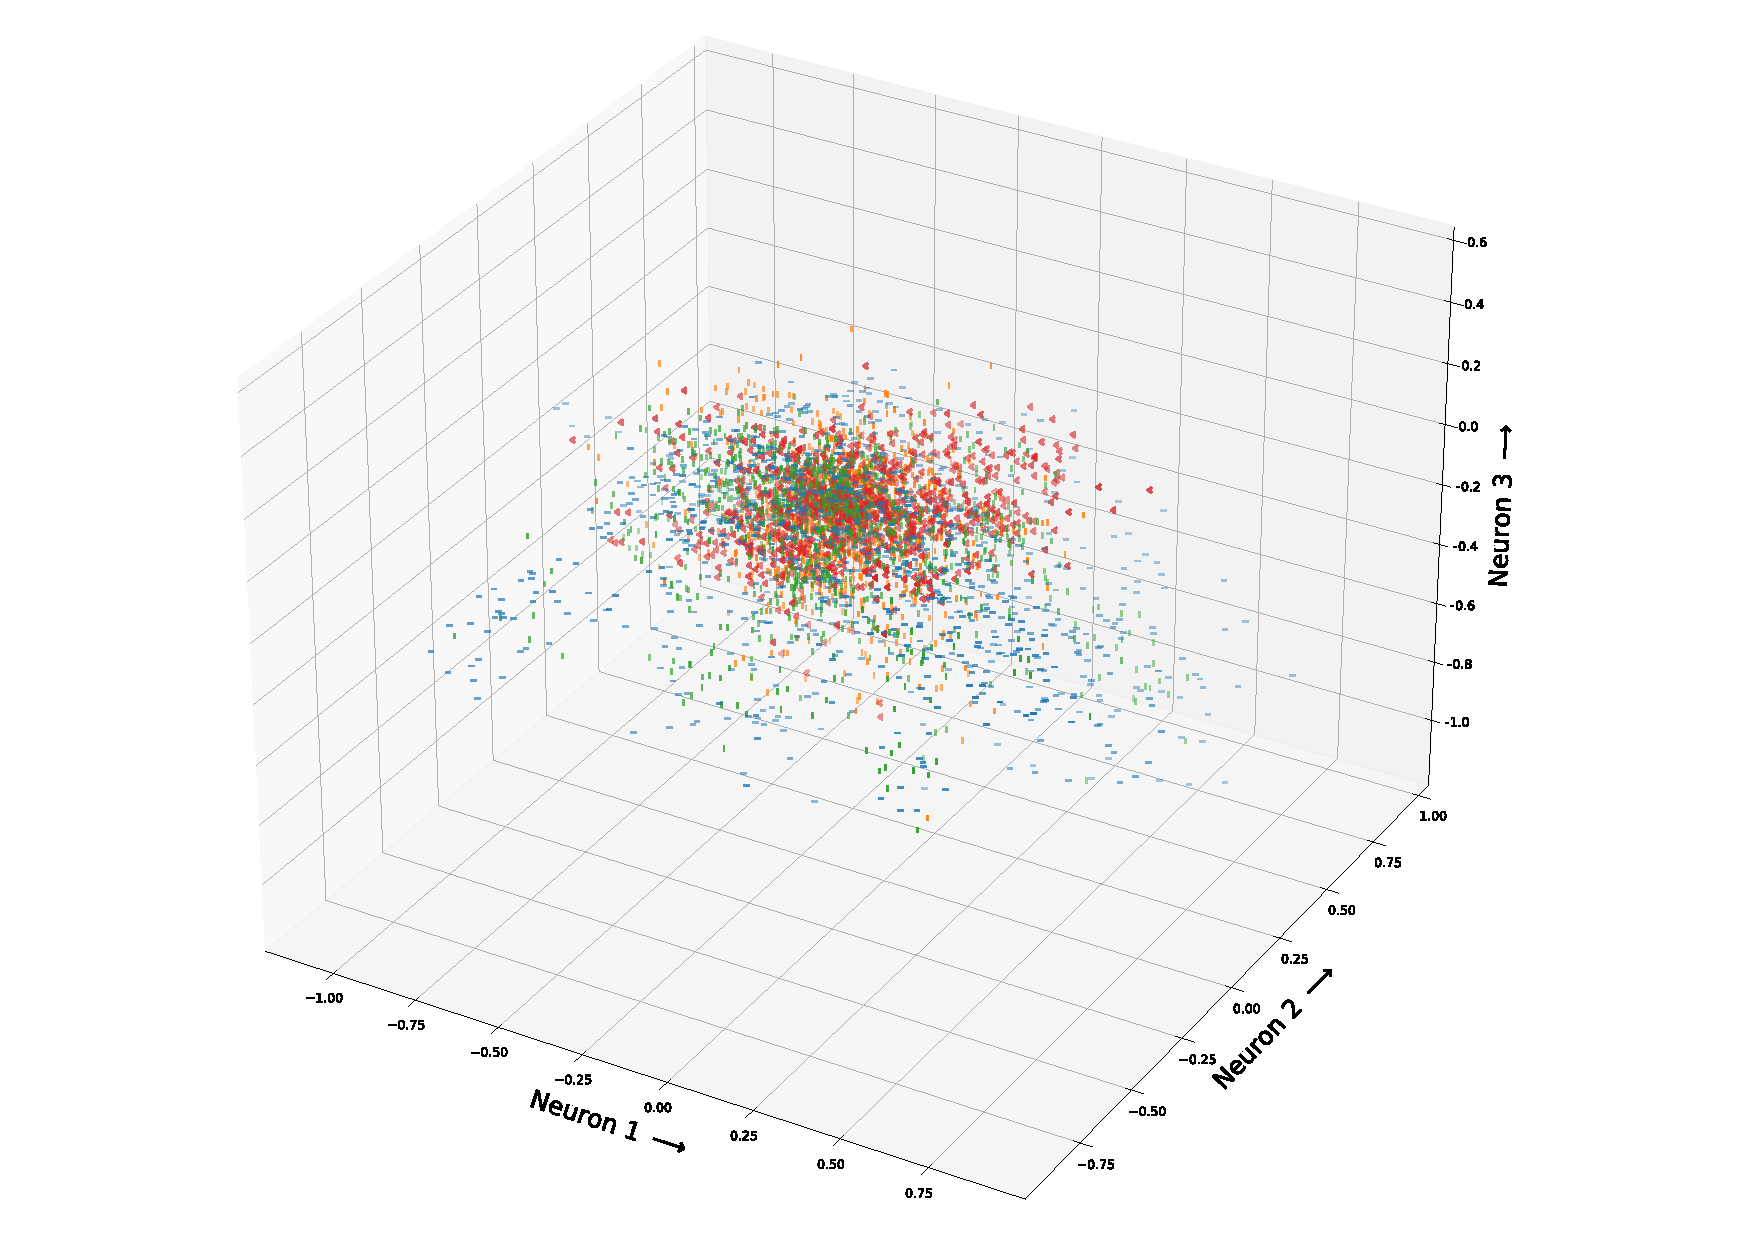
\includegraphics[width=.44\textwidth]{GAMMA_distribution/mmd_epoch0_0_1.pdf}
  \hspace{.3cm}
  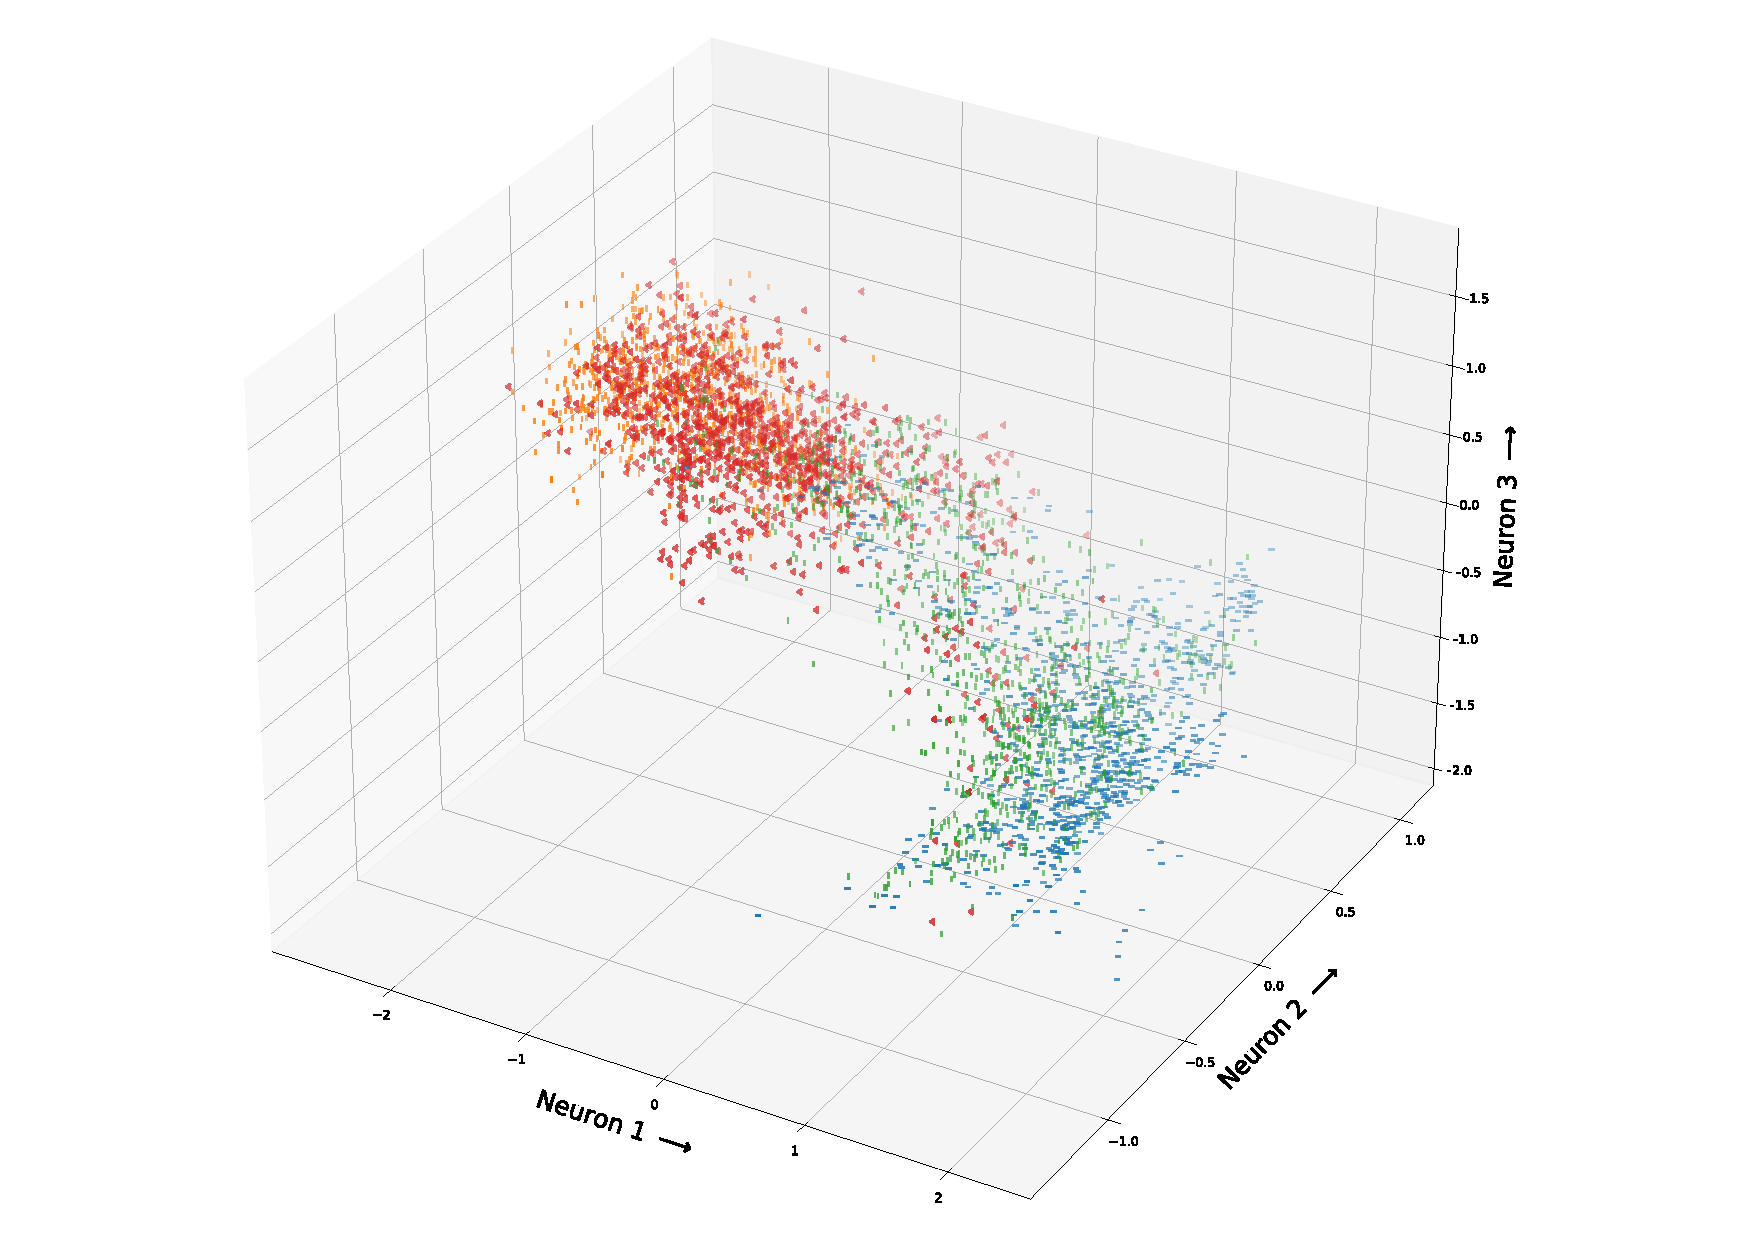
\includegraphics[width=.44\textwidth]{GAMMA_distribution/mmd_epoch8_0_1.pdf}

  \vspace{.1cm}

  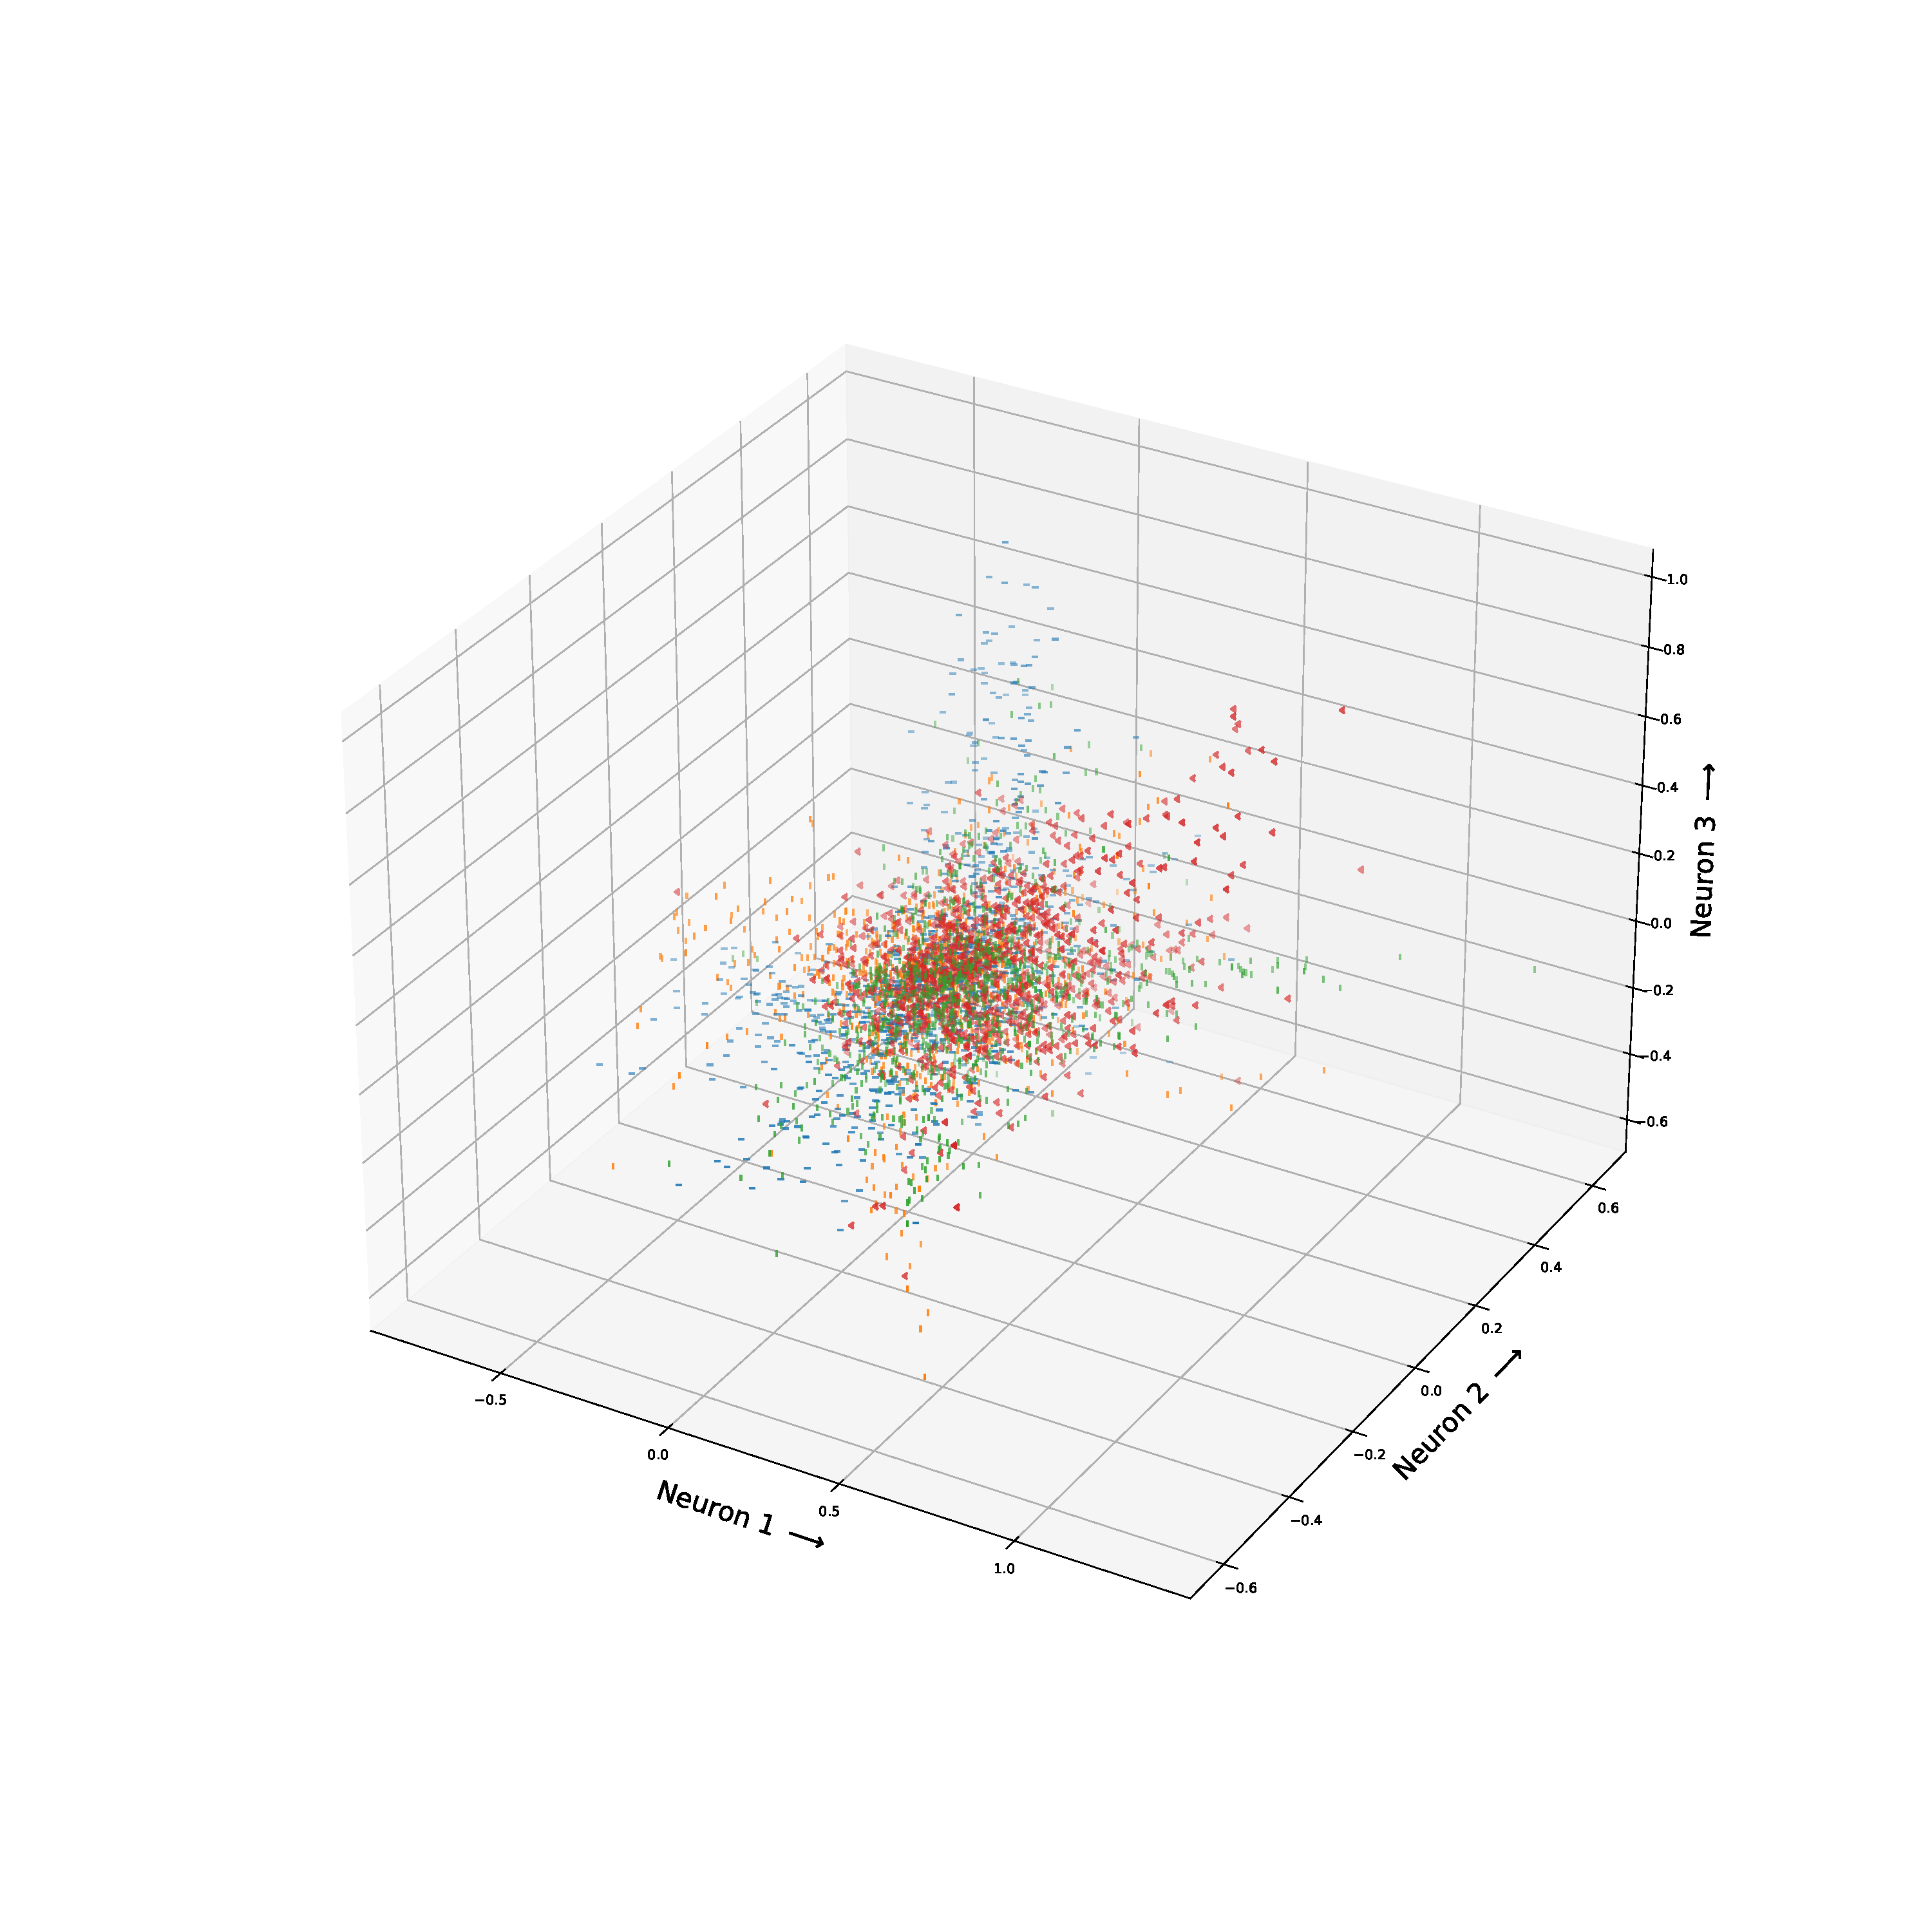
\includegraphics[width=.44\textwidth]{GAMMA_distribution/mmd_epoch0_0_5.pdf}
  \hspace{.3cm}
  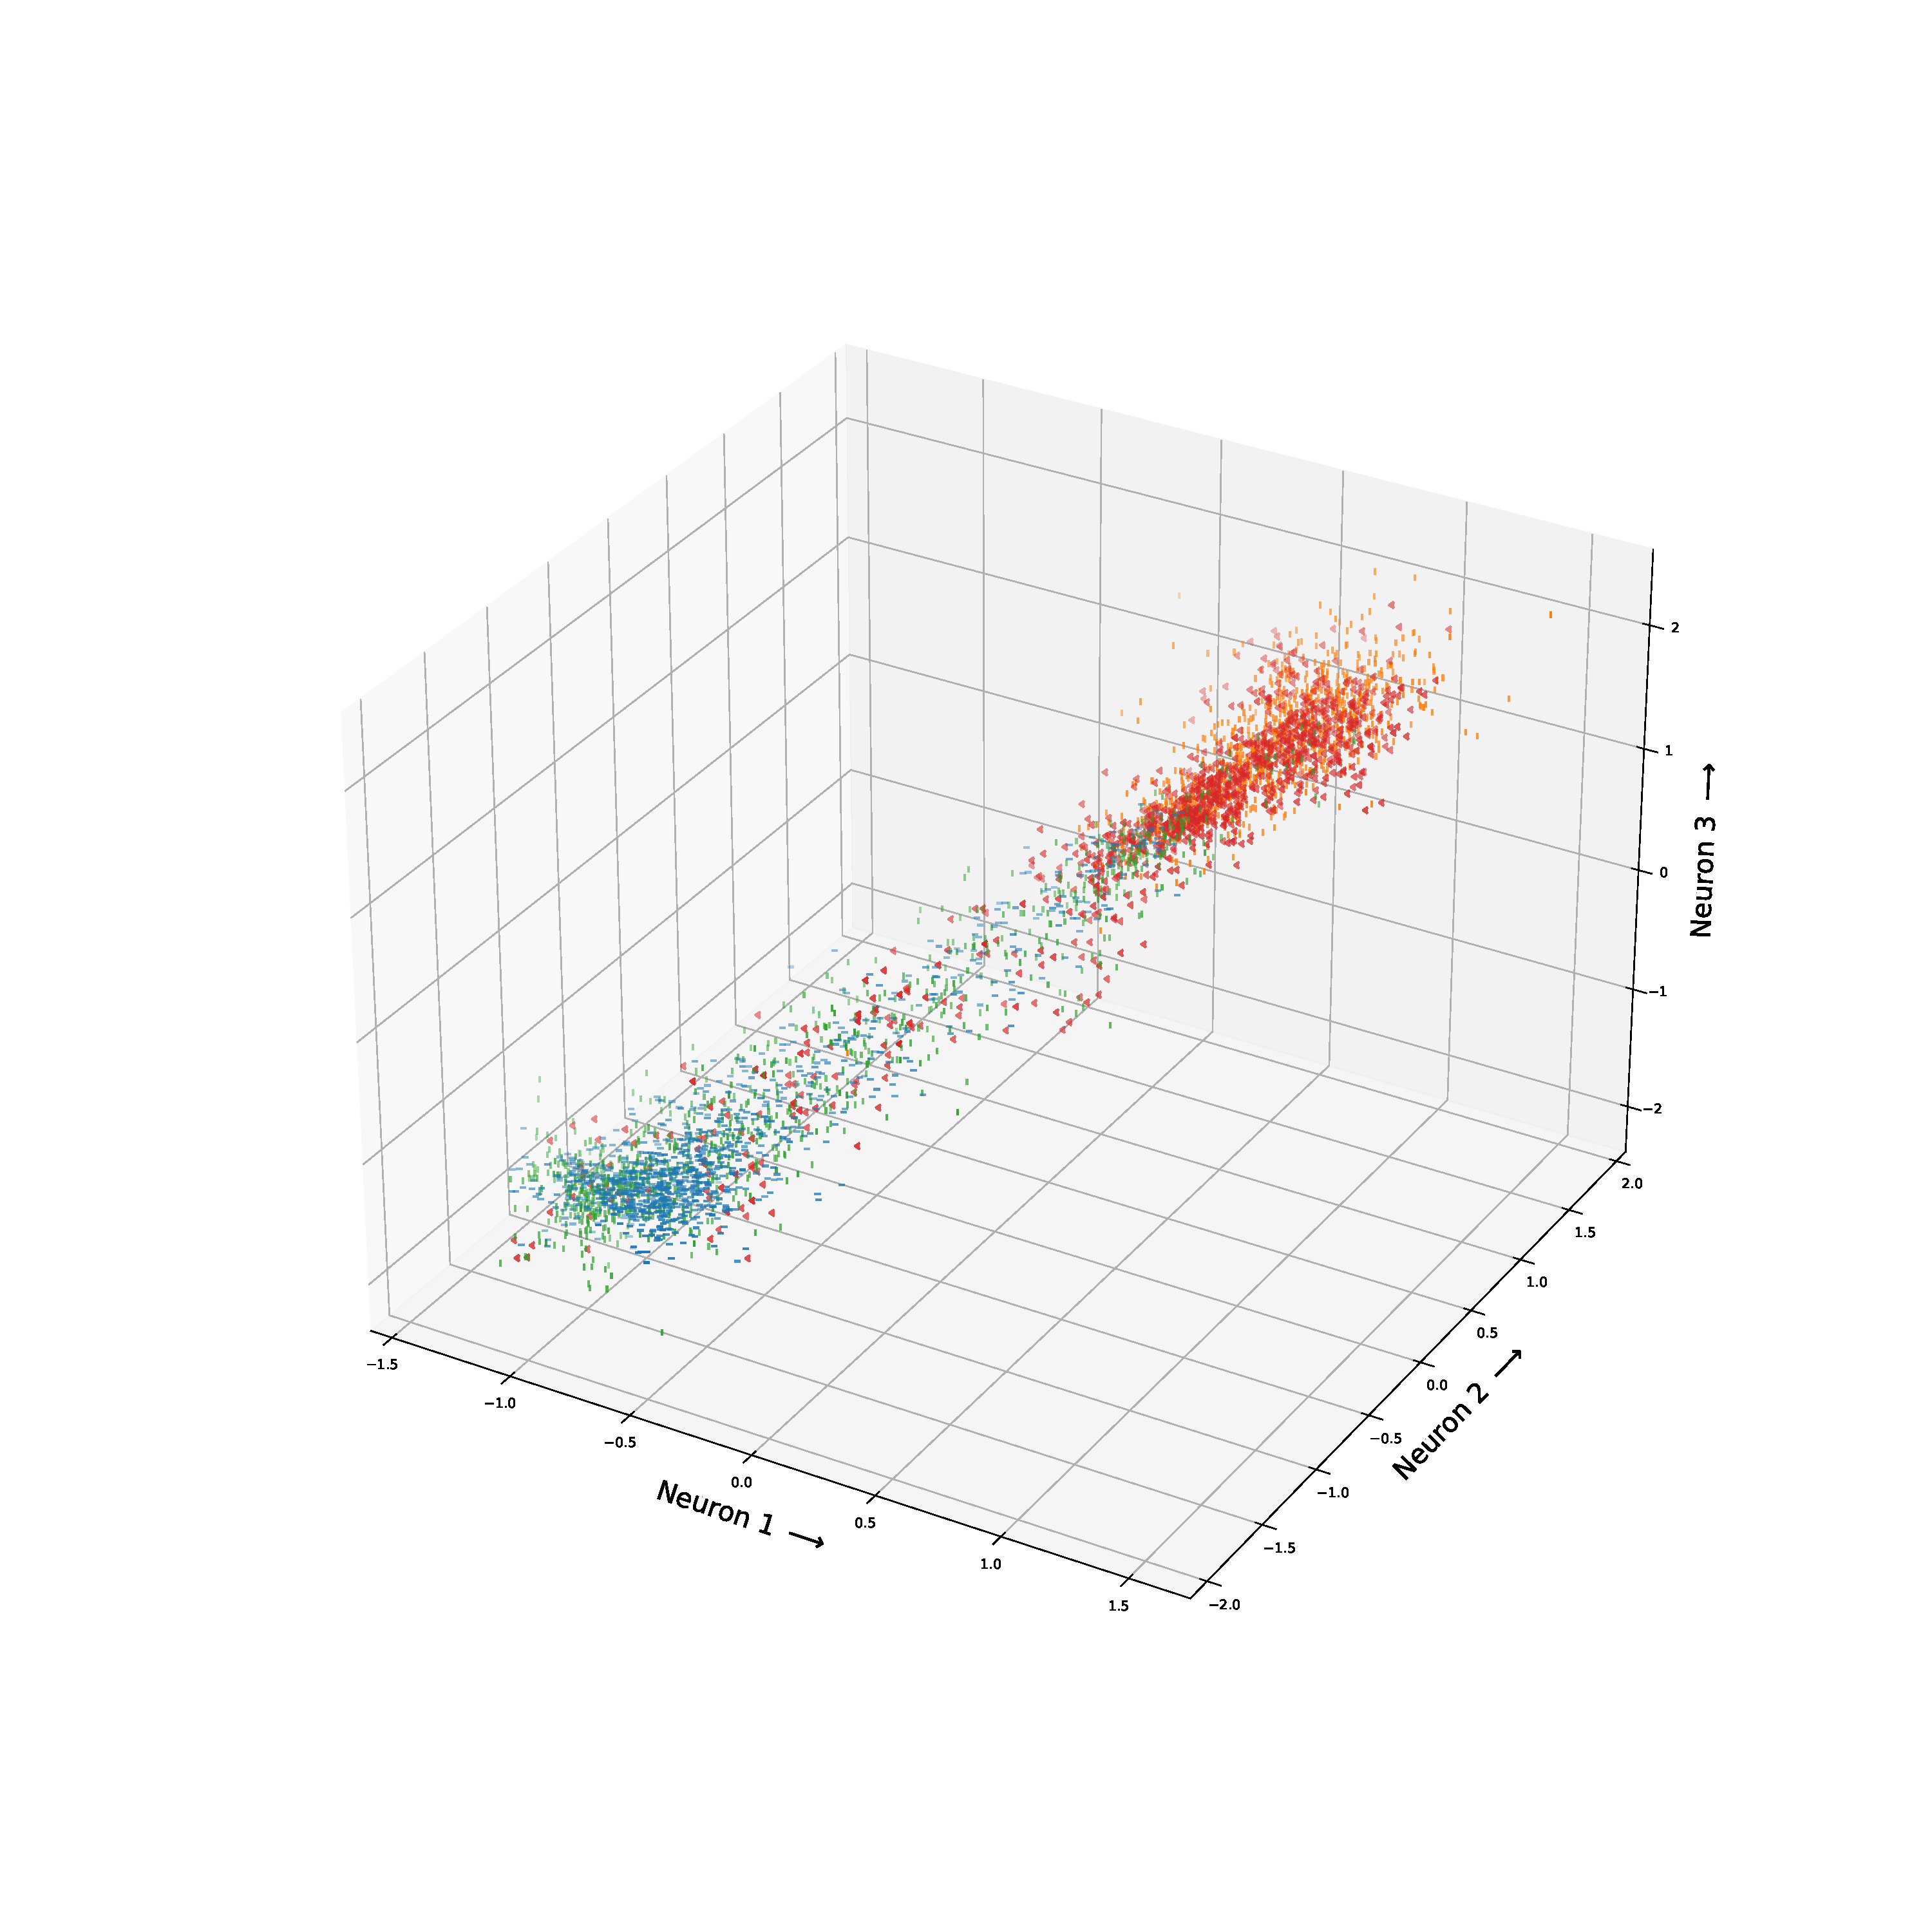
\includegraphics[width=.44\textwidth]{GAMMA_distribution/mmd_epoch8_0_5.pdf}

  \vspace{.1cm}

  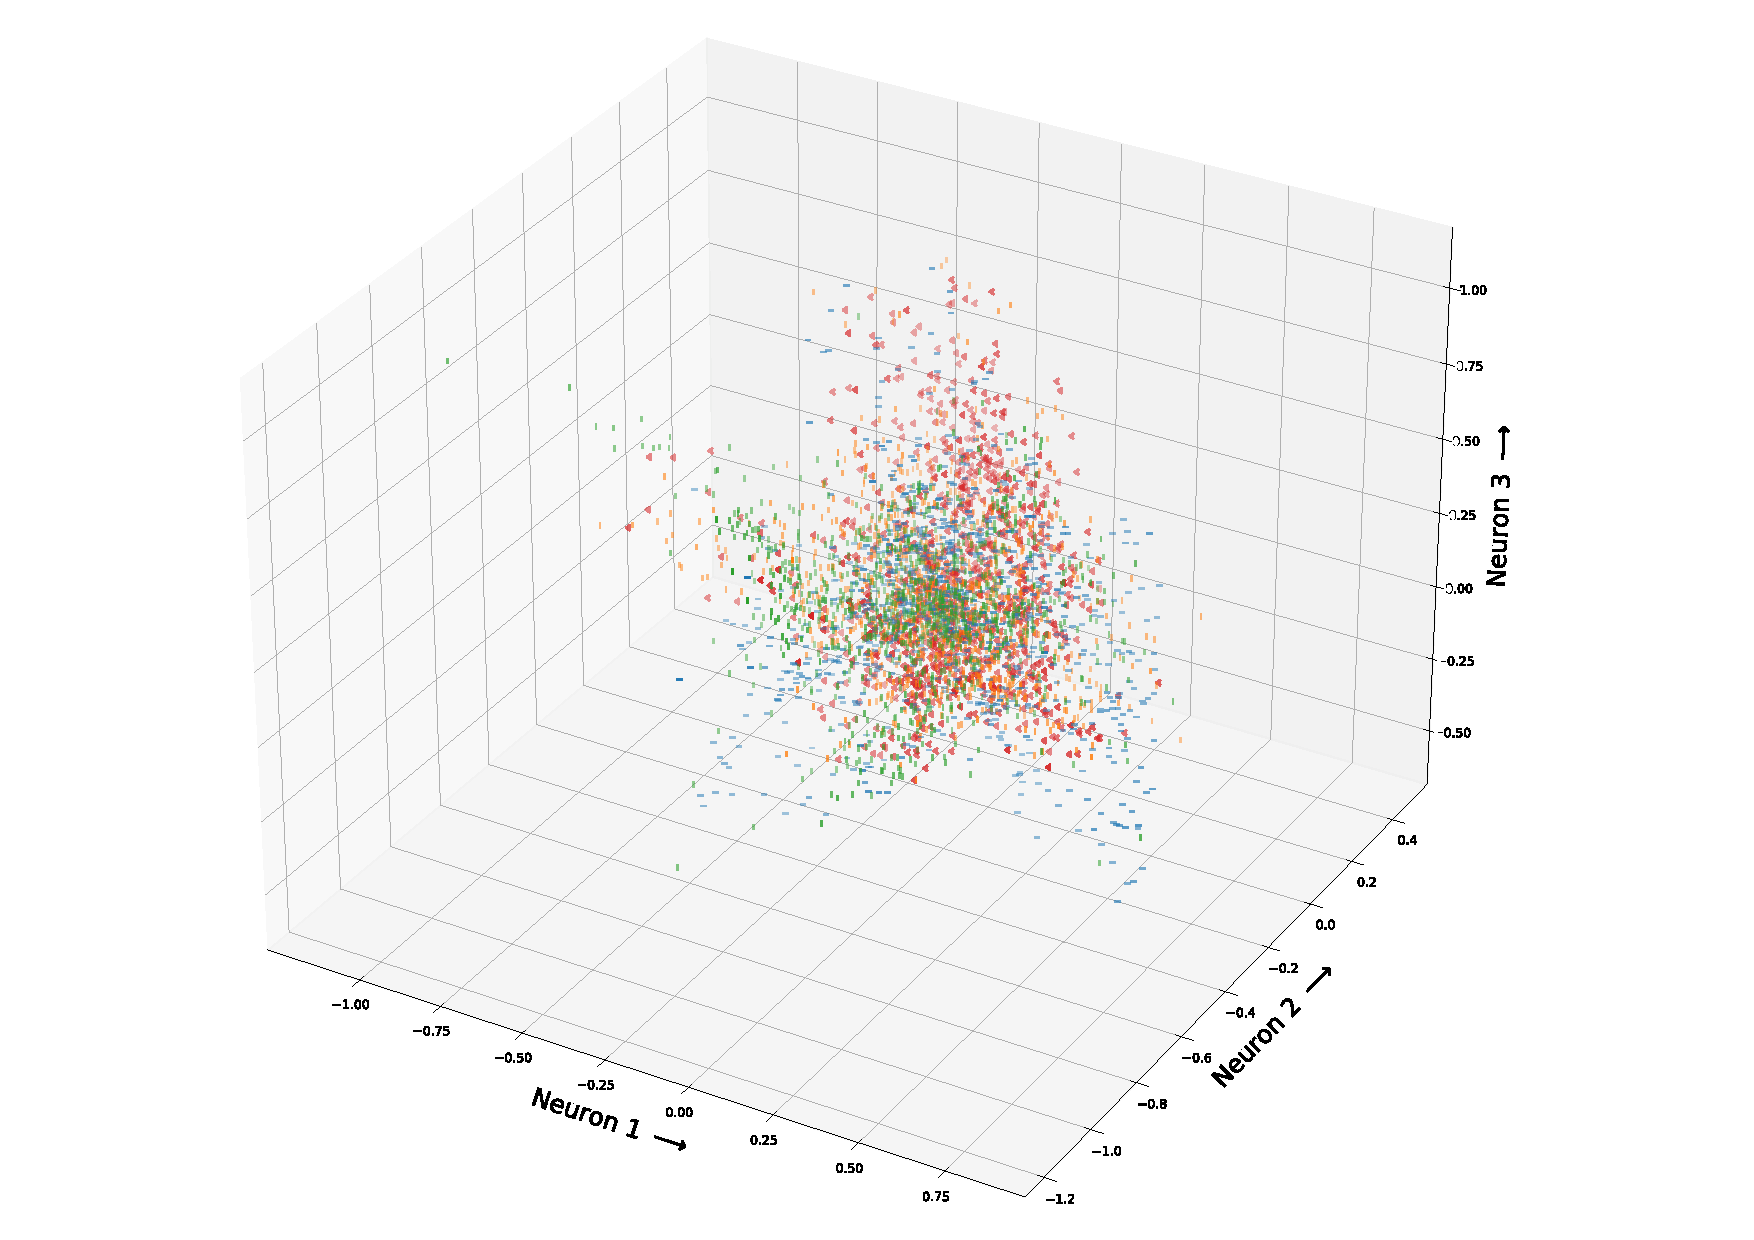
\includegraphics[width=.44\textwidth]{GAMMA_distribution/mmd_epoch0_30.pdf}
  \hspace{.3cm}
  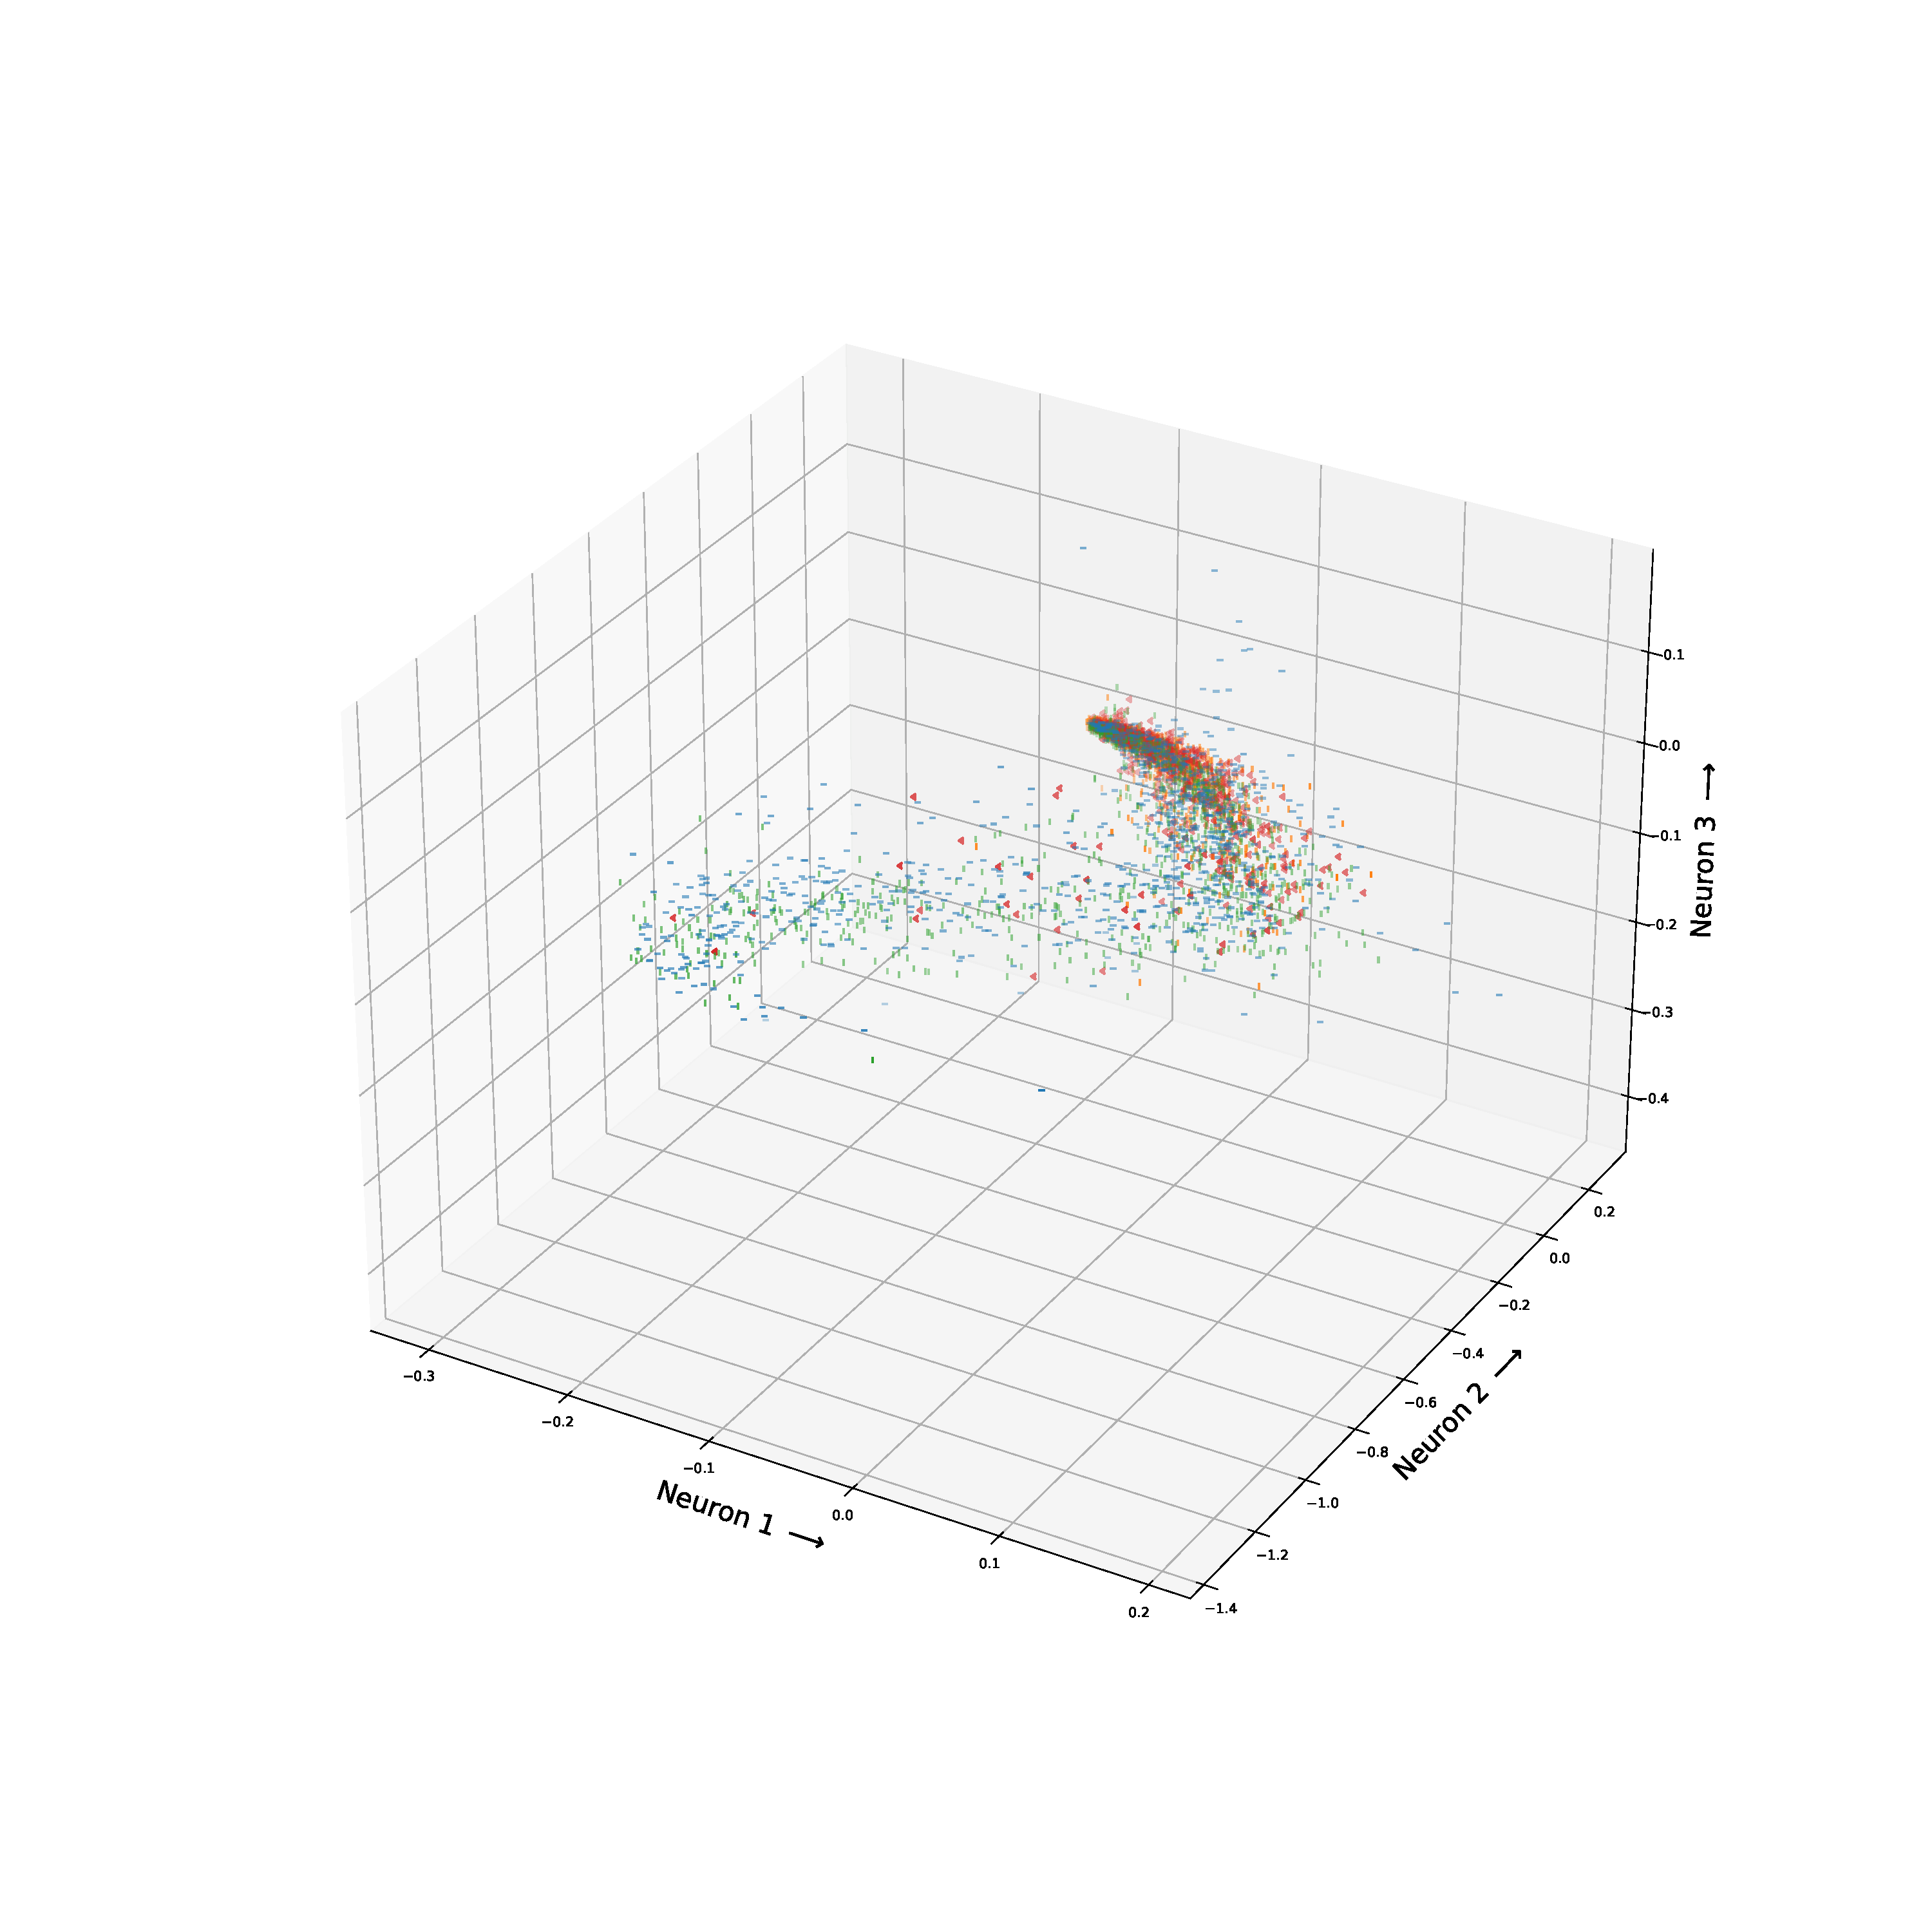
\includegraphics[width=.44\textwidth]{GAMMA_distribution/mmd_epoch8_30.pdf}
  
  \vspace{.1cm}
  
  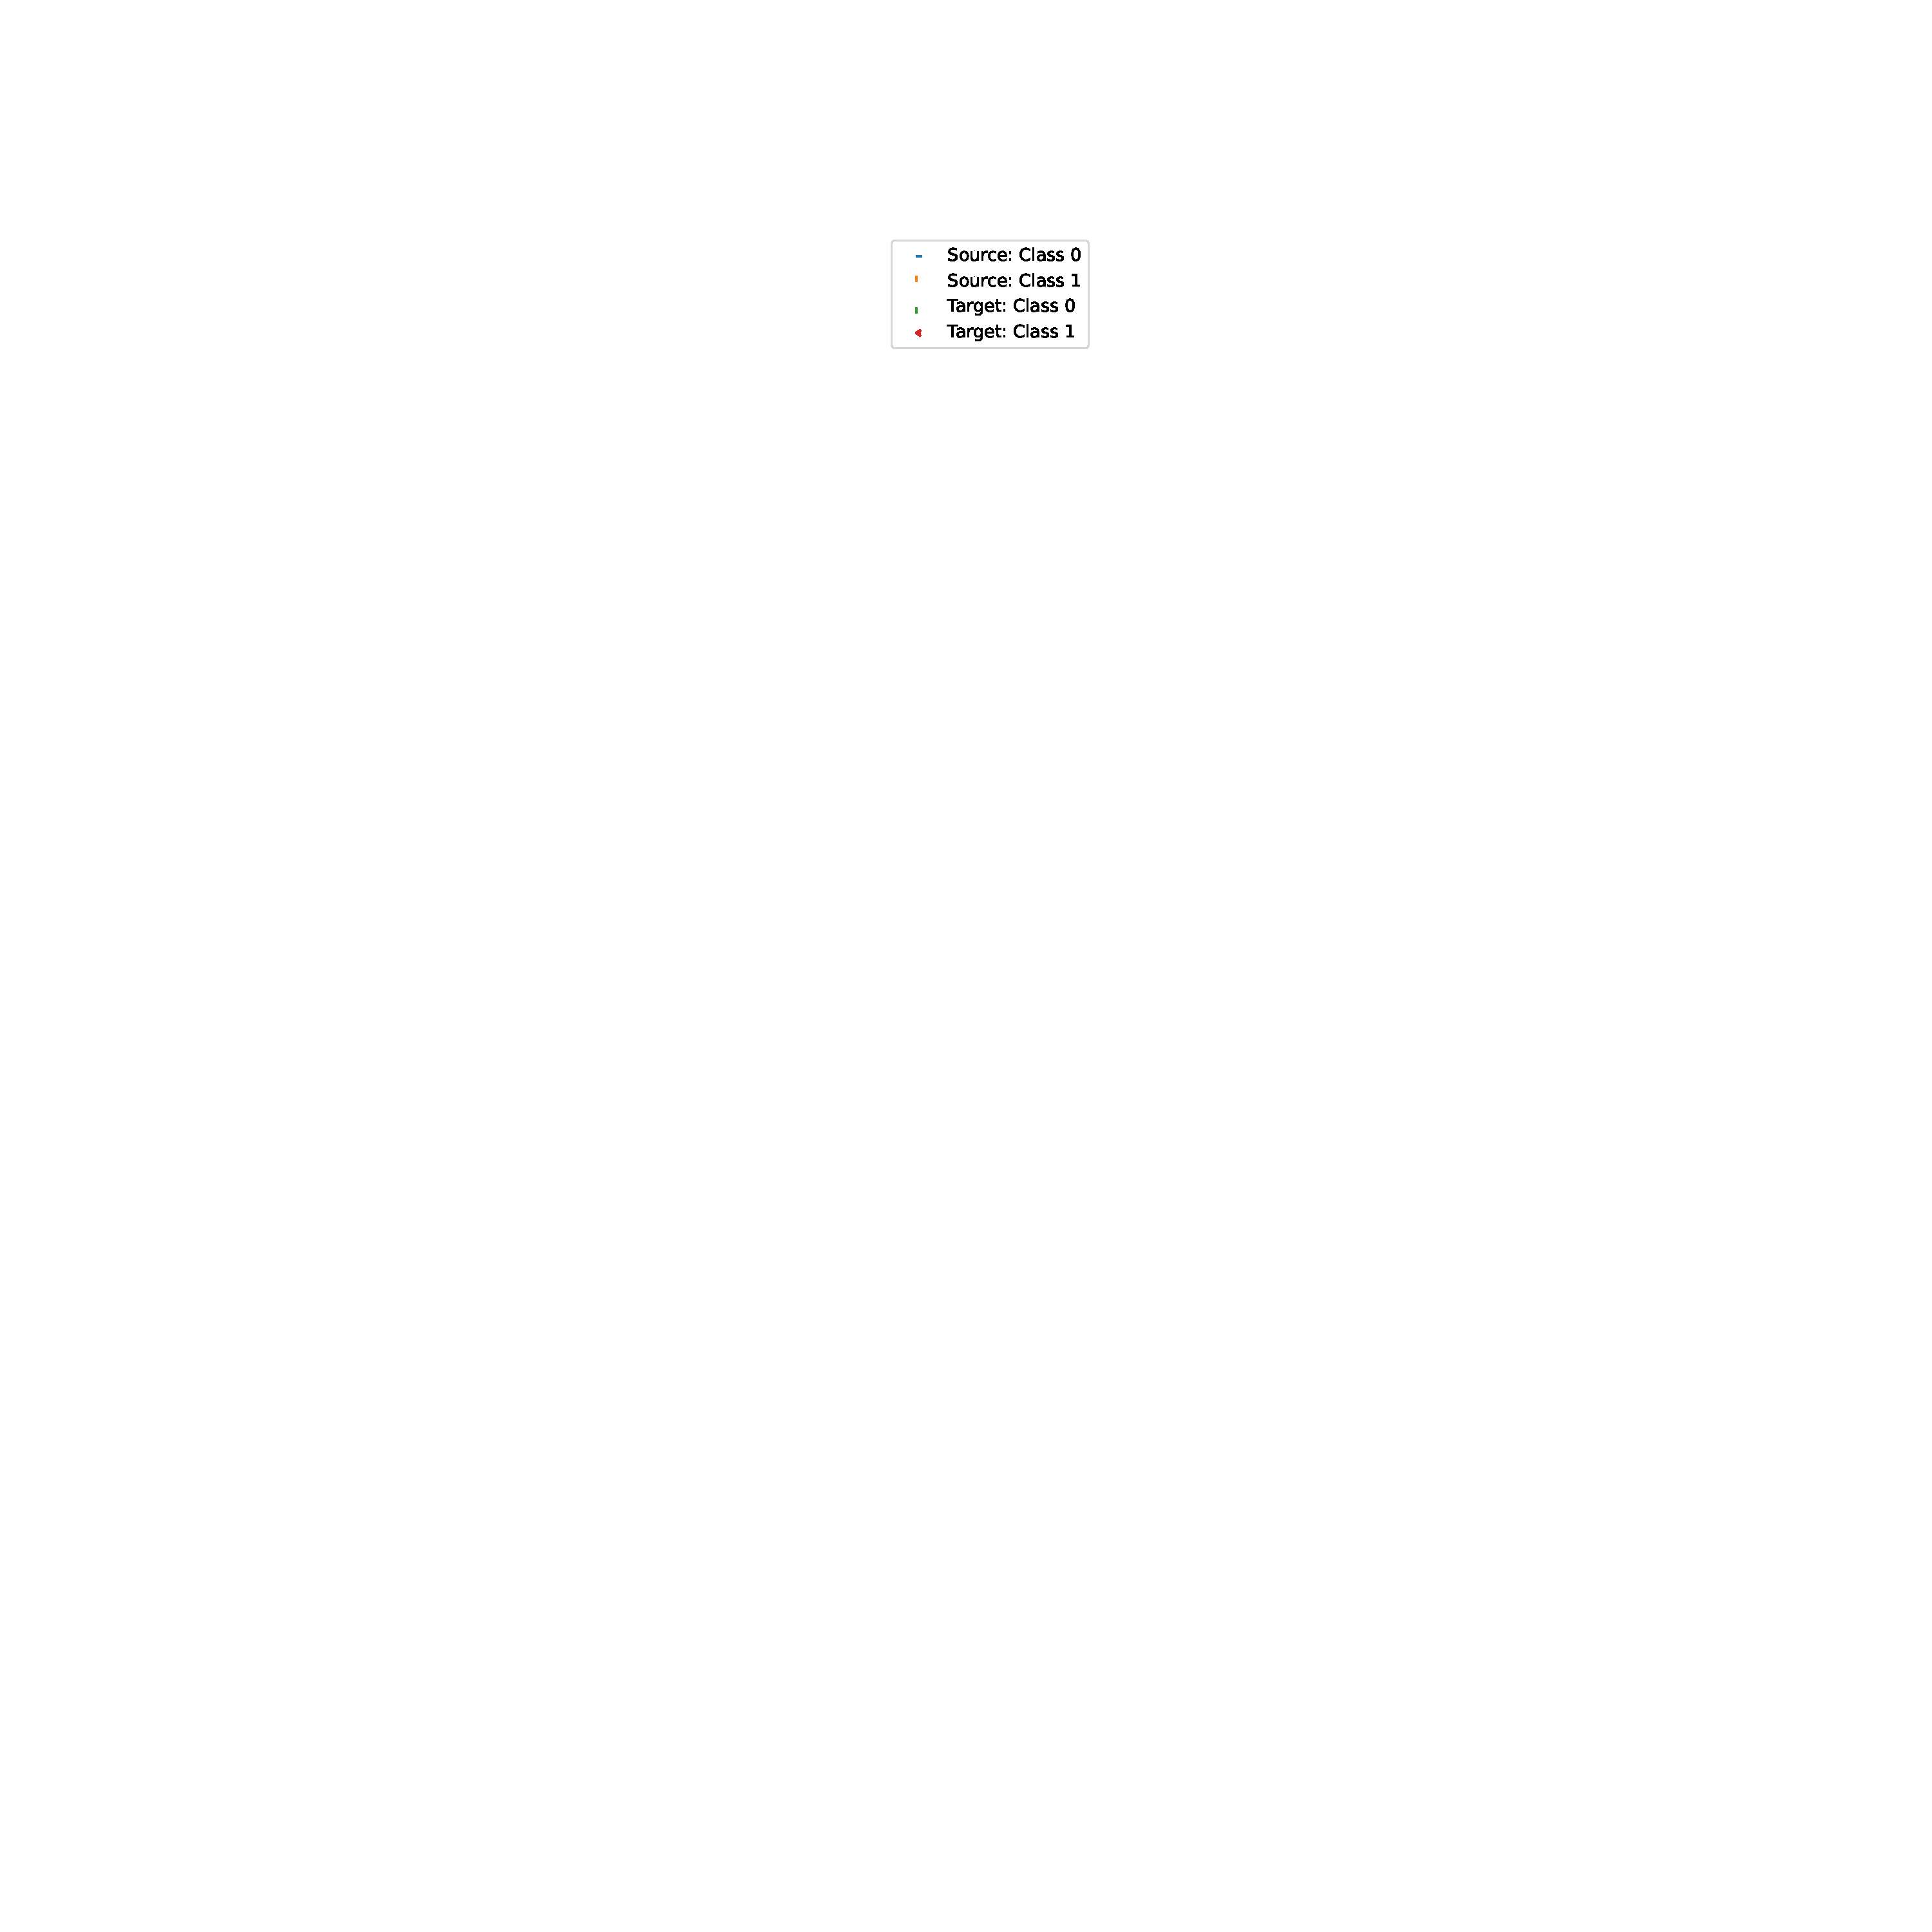
\includegraphics[width=.15\textwidth]{labeled_vs_unlabeled_point_cloud/legend.pdf}


  \caption{Data distribution: Influence of GAMMA on model training, with GAMMA = 0.1 (top), GAMMA = 0,5 (middle), GAMMA = 30 (bottom)}
  \label{fig:point_cloud_mmd}
\end{figure}





\begin{figure}[H]
  \centering
  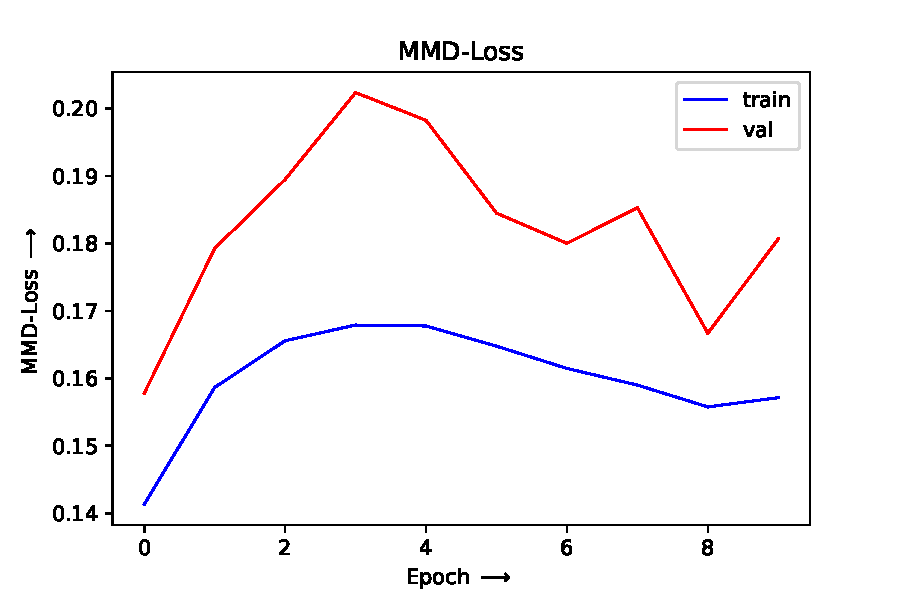
\includegraphics[width=.45\textwidth]{GAMMA_plot/mmd_loss_0_1.pdf}
  \hspace{.3cm}
  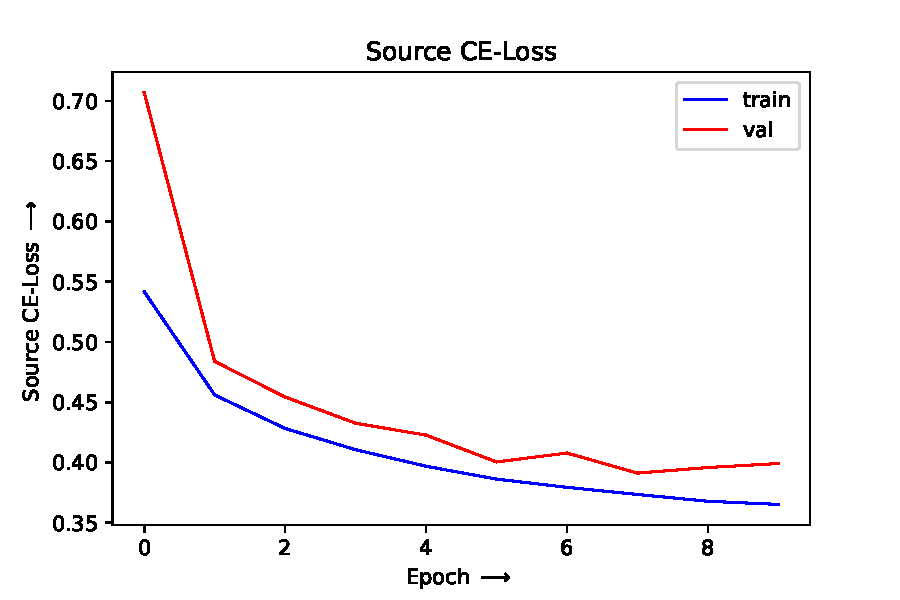
\includegraphics[width=.45\textwidth]{GAMMA_plot/source_ce_loss_0_1.pdf}

  \vspace{.3cm}

  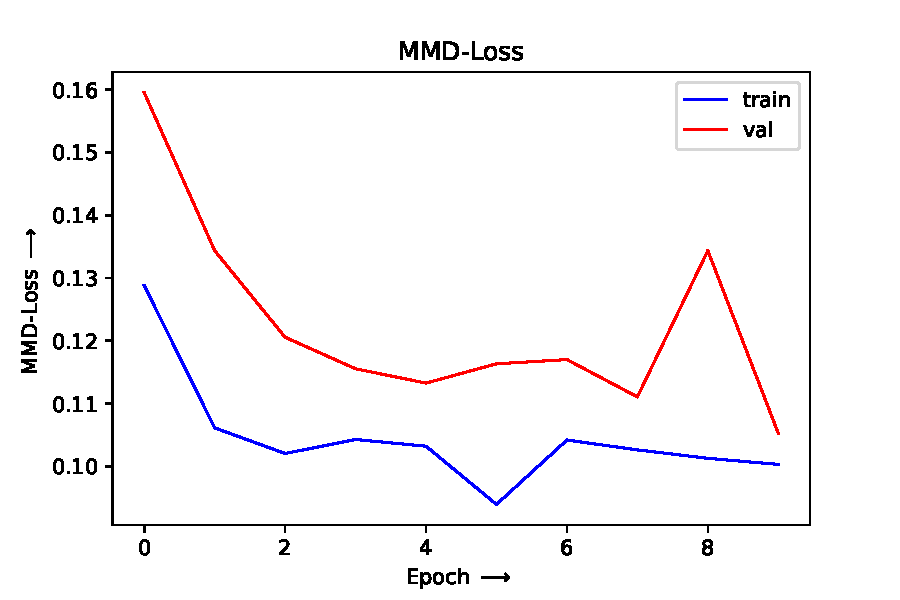
\includegraphics[width=.45\textwidth]{GAMMA_plot/mmd_loss_0_5.pdf}
  \hspace{.3cm}
  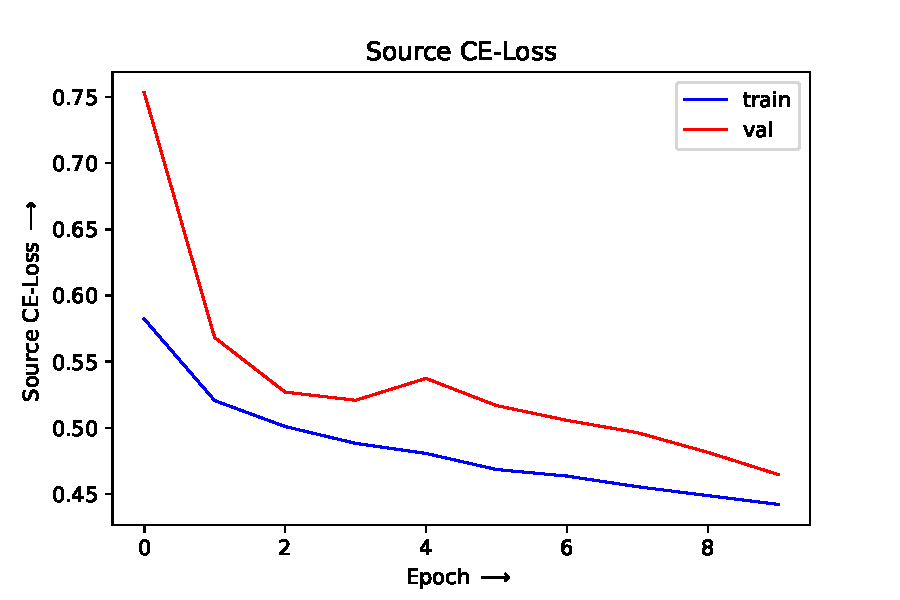
\includegraphics[width=.45\textwidth]{GAMMA_plot/source_ce_loss_0_5.pdf}

  \vspace{.3cm}

  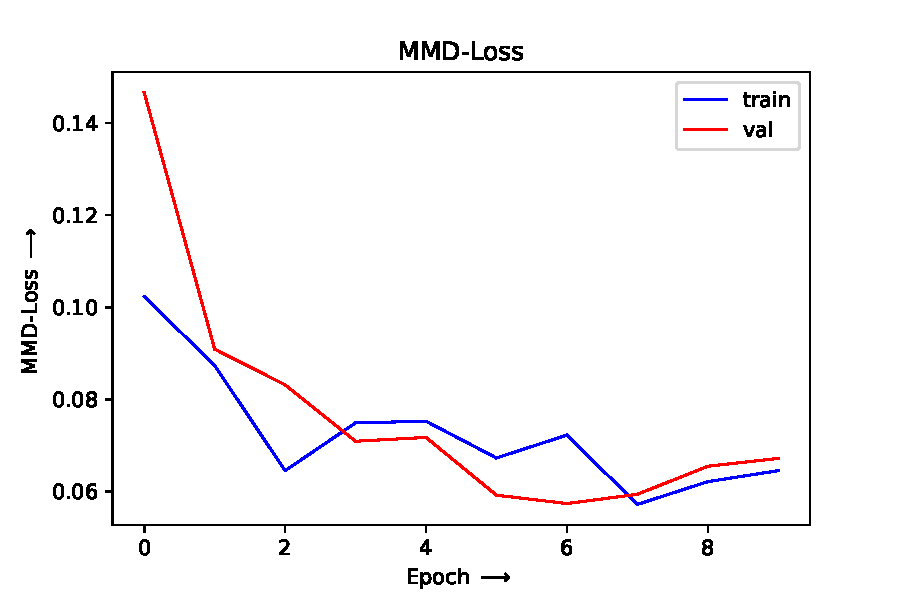
\includegraphics[width=.45\textwidth]{GAMMA_plot/mmd_loss_30.pdf}
  \hspace{.3cm}
  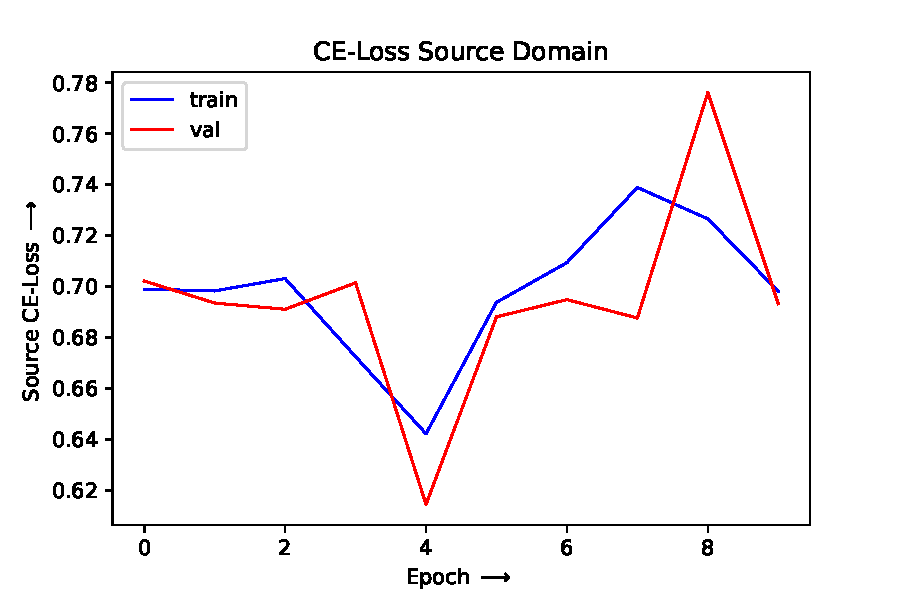
\includegraphics[width=.45\textwidth]{GAMMA_plot/source_ce_loss_30.pdf}

  \caption{MMD and Source CE-Loss curves: Influence of GAMMA on model training, with GAMMA = 0.1 (top), GAMMA = 0,5 (middle), GAMMA = 30 (bottom)}
  \label{fig:learning_curves_influence_mmd_feature_extractor}
\end{figure}

Just when the GAMMA is chosen carefully the source cross-entropy and MMD loss can be reduced. For the other just mentioned cases either either the MMD or source cross-entropy loss could not be reduced during the training. Bedsides that, one can see how the samples are distributed a lot more equally and how the compactness and separability of the classes is increased for both domains. For extreme GAMMA choices the optimization just focuses on one of the two losses and therefore training goals. In the case of a big GAMMA, the model does not learn to predict classes correctly, but just tries to reduce the distance between the samples of all classes and domains. If GAMMA is picked to small the model is able to predict the the source domain labels accurately but can not transfer that knowledge to the target domain. 

\subsection{Labeled vs. unlabeled MMD loss} \label{sec:Differences of labeled and unlabeled MMD loss}

The idea behind domain adaption is to aggregate knowledge while solving one problem and transferring that knowledge to another problem. For this reason in domain adaption tasks the goal is to restrict the supervised learning solely on the source domain data. Section \ref{sec:Balancing Cross-Entropy and MMD loss} describes how applying the MMD loss in general can reduce the domain discrepancy. Since the target labels are unknown the intra- and inter-class distance between source and target samples is minimized. Obviously this also reduces the separability of classes for both domains. In the literature domain adaption approaches which use a small amount of the target domain labels are known as "Few-shot transfer learning" \cite{WU2020}. Similarly in this section the effect of including a few target labels into the training is analysed. The cross-entropy loss is still restricted to the source domain. Solely the MMD loss is allowed to use the target labels. This allows to calculate the distance between source and target samples of similar and of different classes separately. The labeled MMD loss optimizes the model such, that the intra-class distance between the domains is maximized and the inter-class distance is minimized. The domain discrepancy is reduced by minimizing the the inter-class distance. The separability is improved by maximizing the the intra-class distance. In parallel the training still includes the source cross-entropy loss in order to improve the source domain classification task. The hyperparameters GAMMAIntraClass and GAMMAInterClass are used to balance the training scope of reducing the inter-class, maximizing the intra-class distance while improving the source domain classification problem:

\begin{equation}
\begin{split}
    TotalMMDLoss = GAMMAIntraClass * MMDLossIntraClass\\ + GAMMAInterClass * MMDLossInterClass + CELoss
\end{split}
\end{equation}

 The MMD loss which includes the target labels is named "labeled MMD loss" and otherwise "unlabeled MMD loss". Again fig. \ref{fig:point_cloud_labeled_unlabeled_mmd} visualizes the distribution of the latent feature representation distribution of the source and target samples within the penultimate hidden layer. Throughout the training both MMD losses reduce the domain discrepancy and increase the separability between classes of both domains. Compared to the unlabeled, the labeled MMD loss is able to increase the distance between the classes of both domains. This increased cross-domain class separability and compactness simplifies the classification problem. Besides that, the model is less prone to be optimized to the trivial solution, in which the latent feature representation of all samples collapse at one point or a needle-like subspace. In this experiment 20\% of target labels were used during the training with the labeled MMD loss. The rest of the training data was processed by a cross-entropy loss.

\begin{figure}[H]
  \centering
  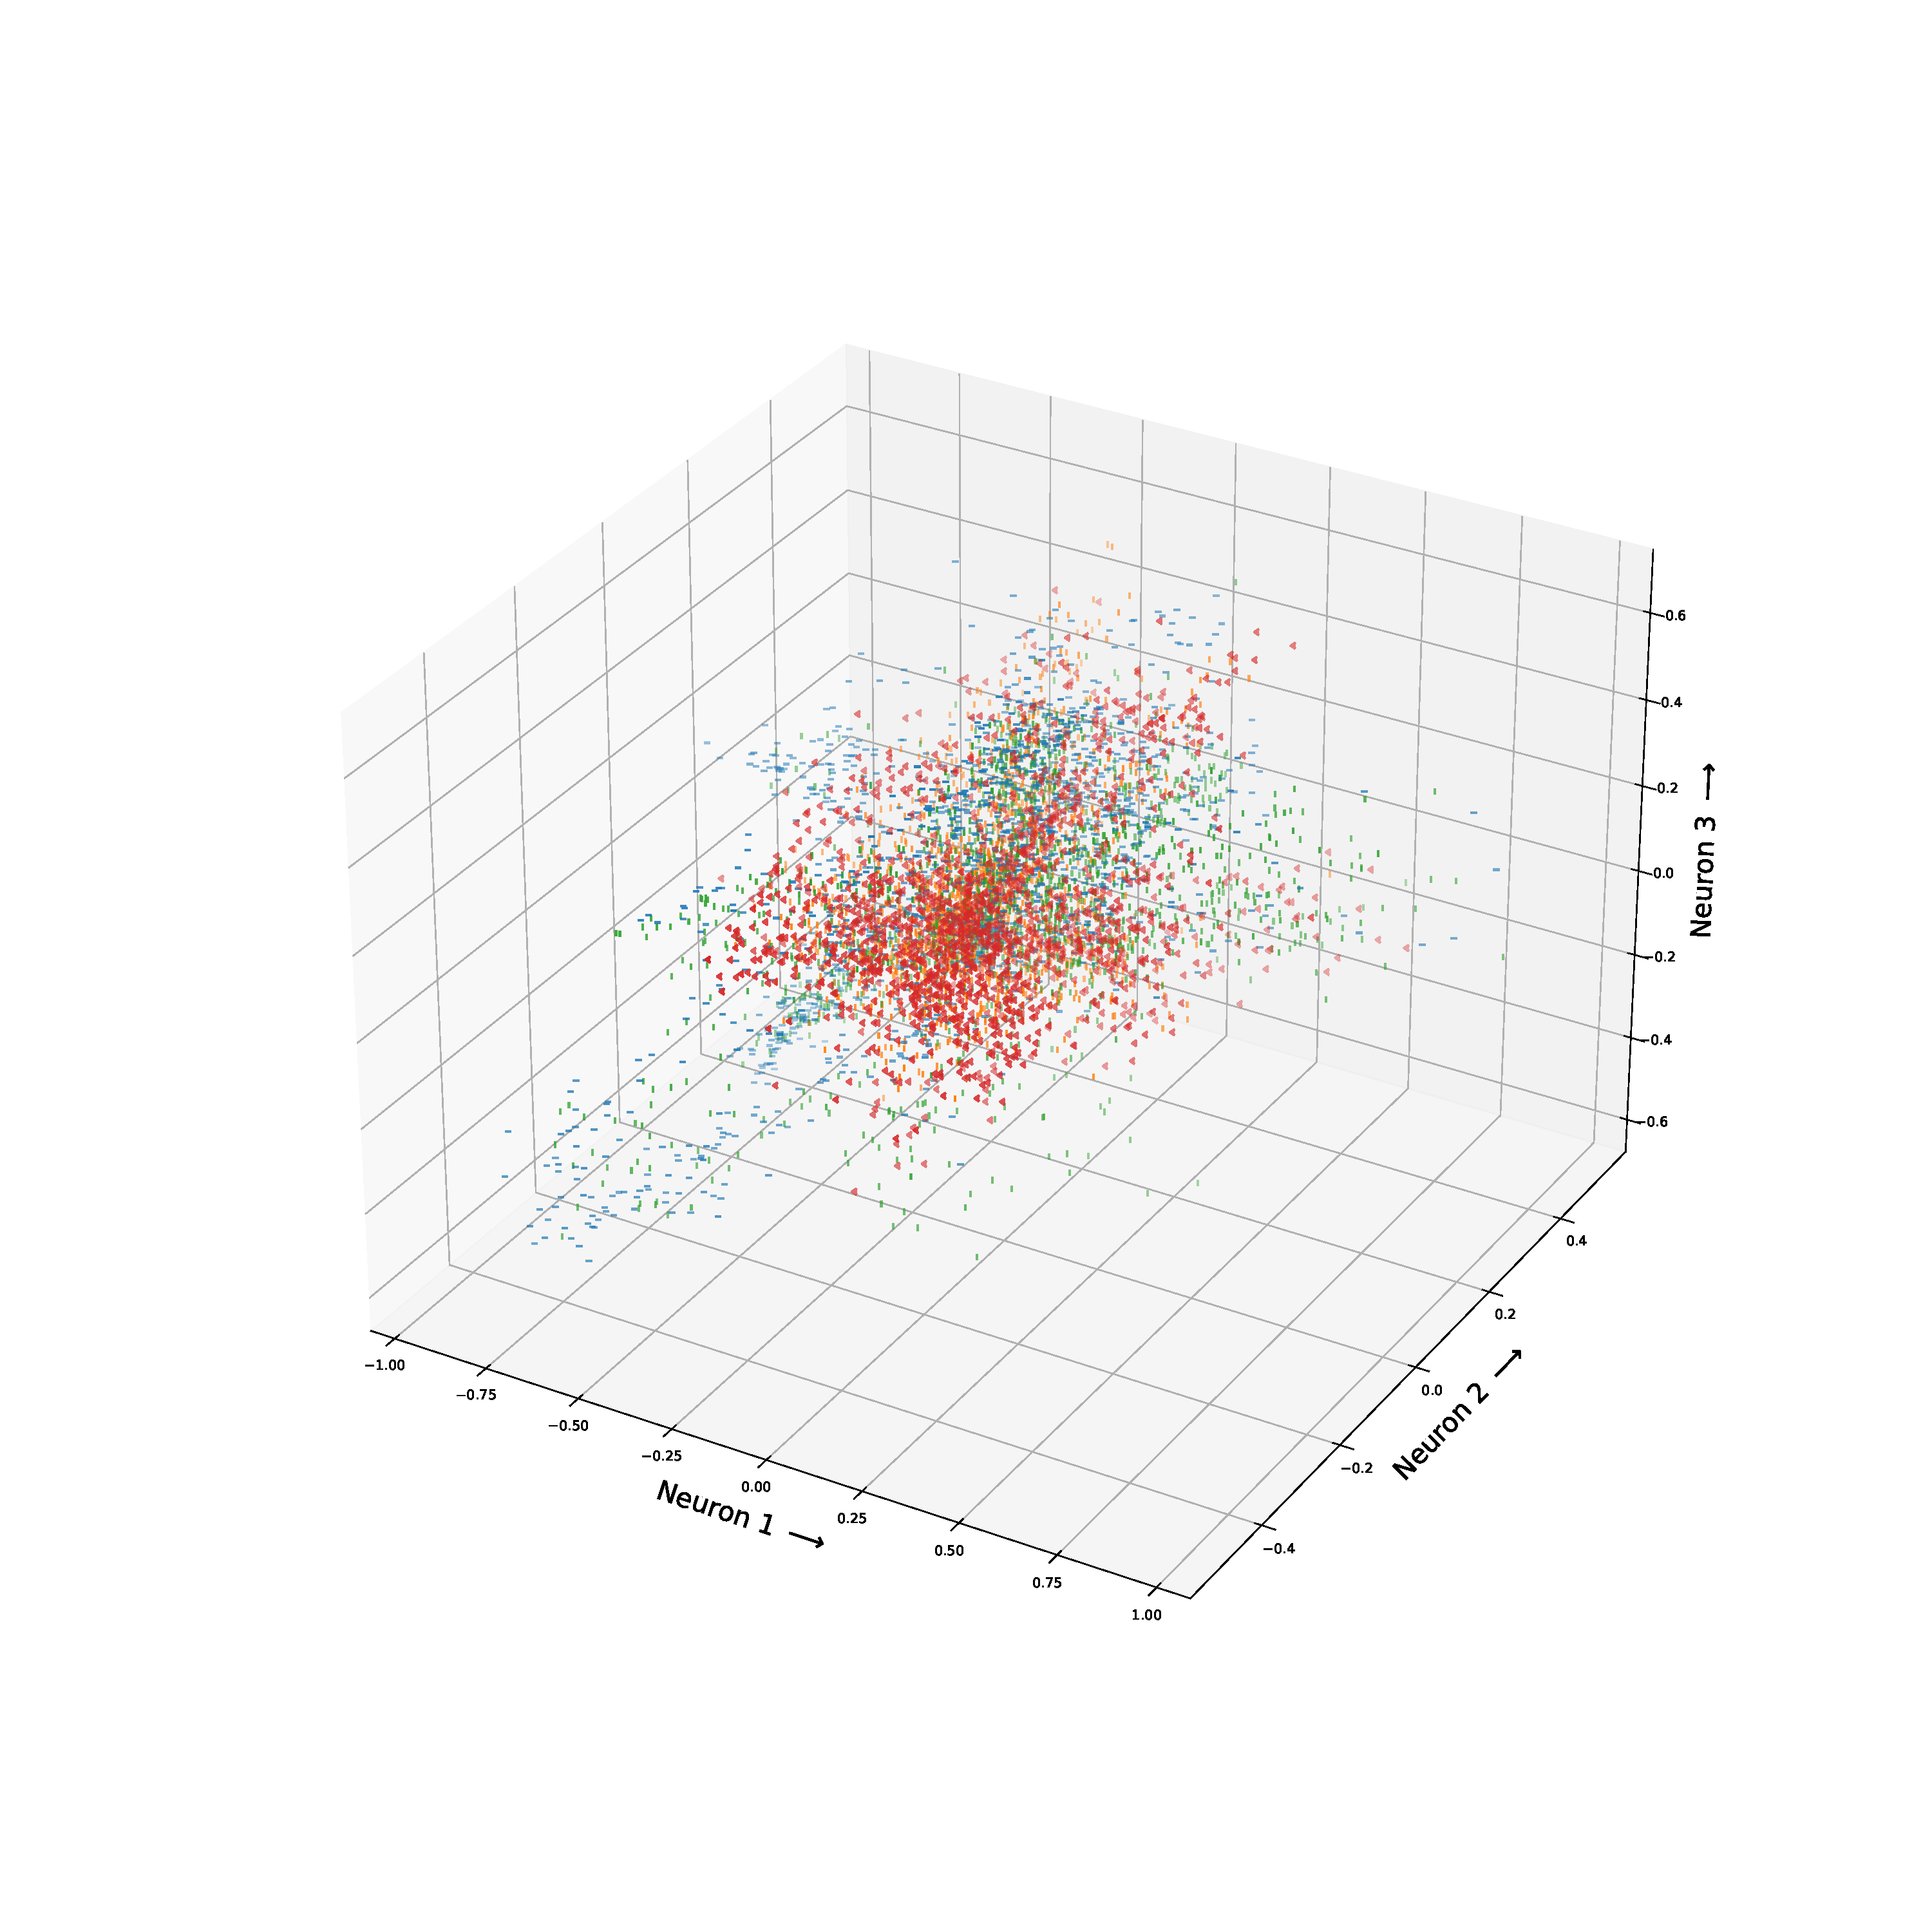
\includegraphics[width=.44\textwidth]{labeled_vs_unlabeled_point_cloud/labeled_mmd_epoch0.pdf}
  \hspace{.3cm}
  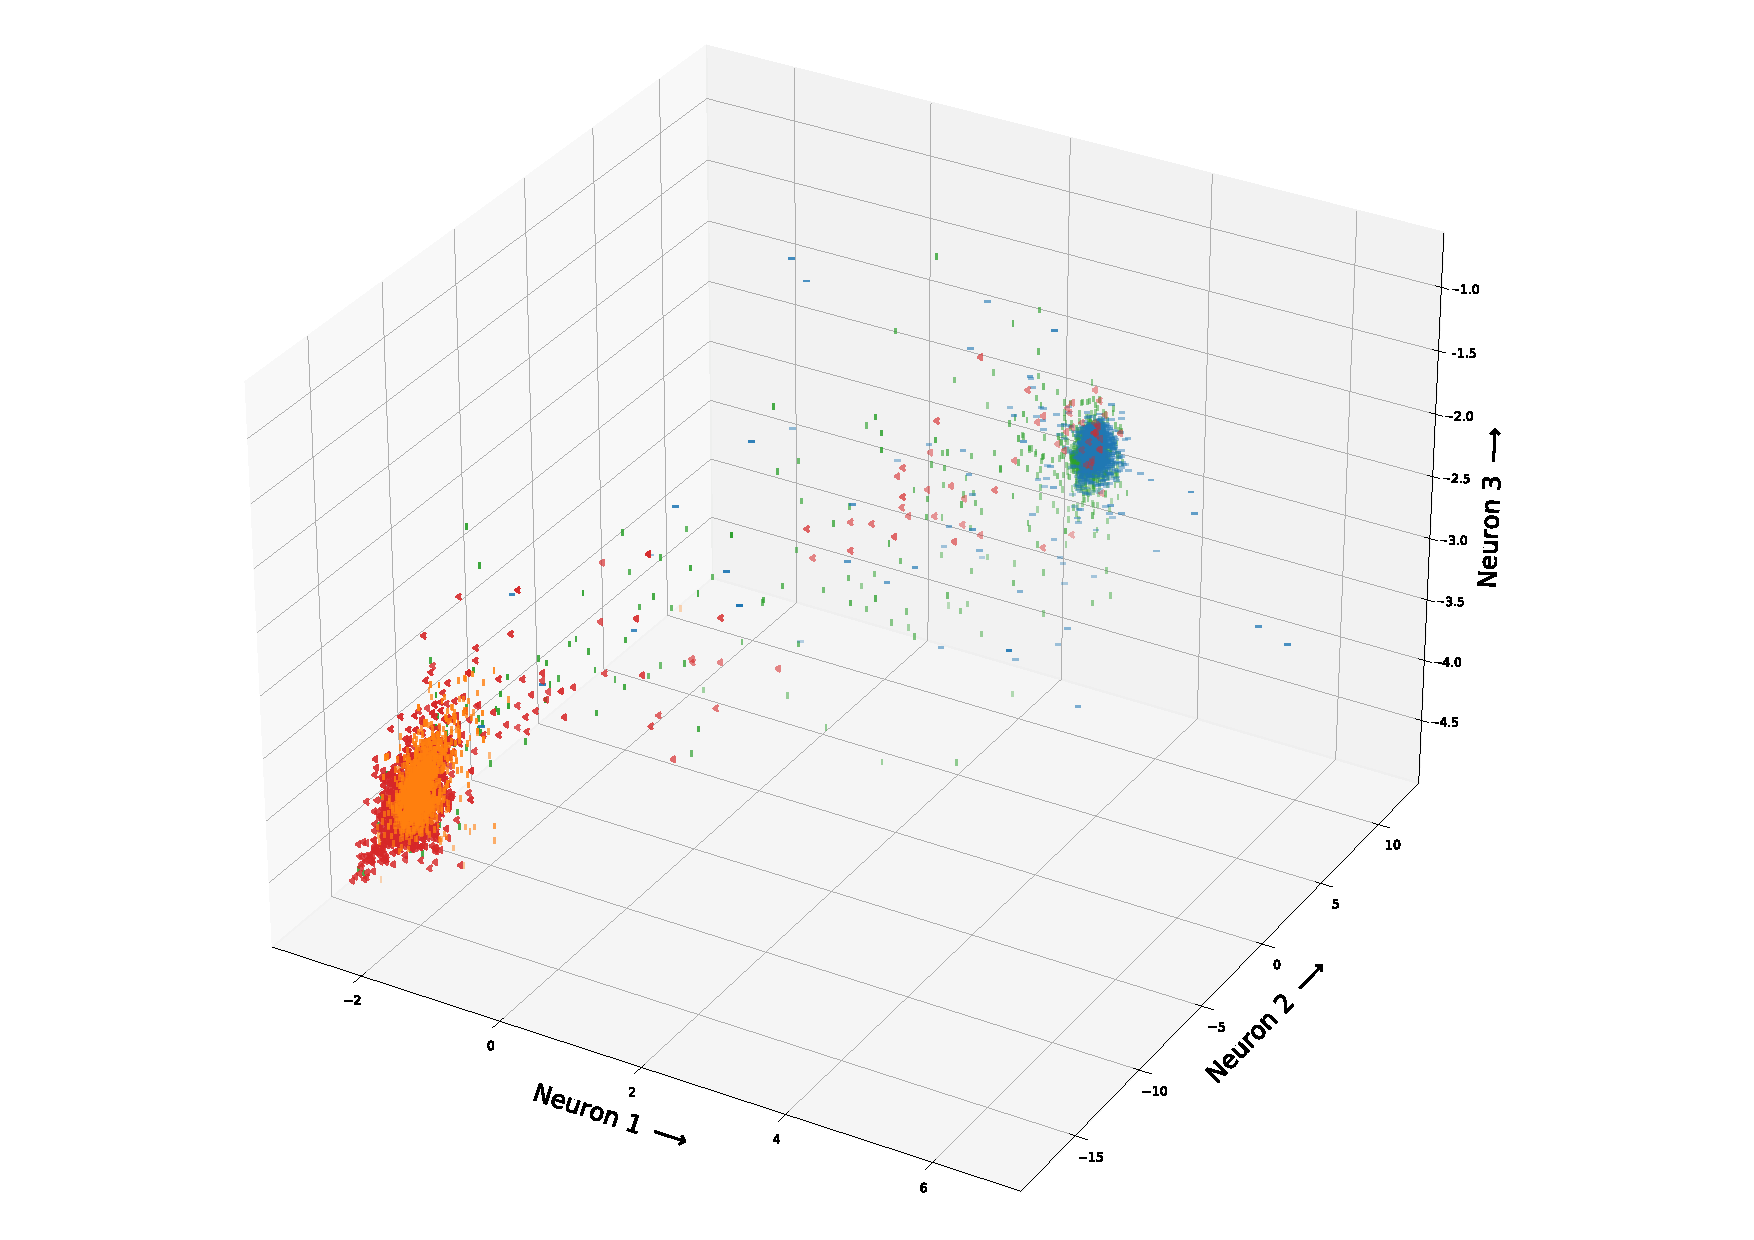
\includegraphics[width=.44\textwidth]{labeled_vs_unlabeled_point_cloud/labeled_mmd_epoch6.pdf}

  \vspace{.1cm}

  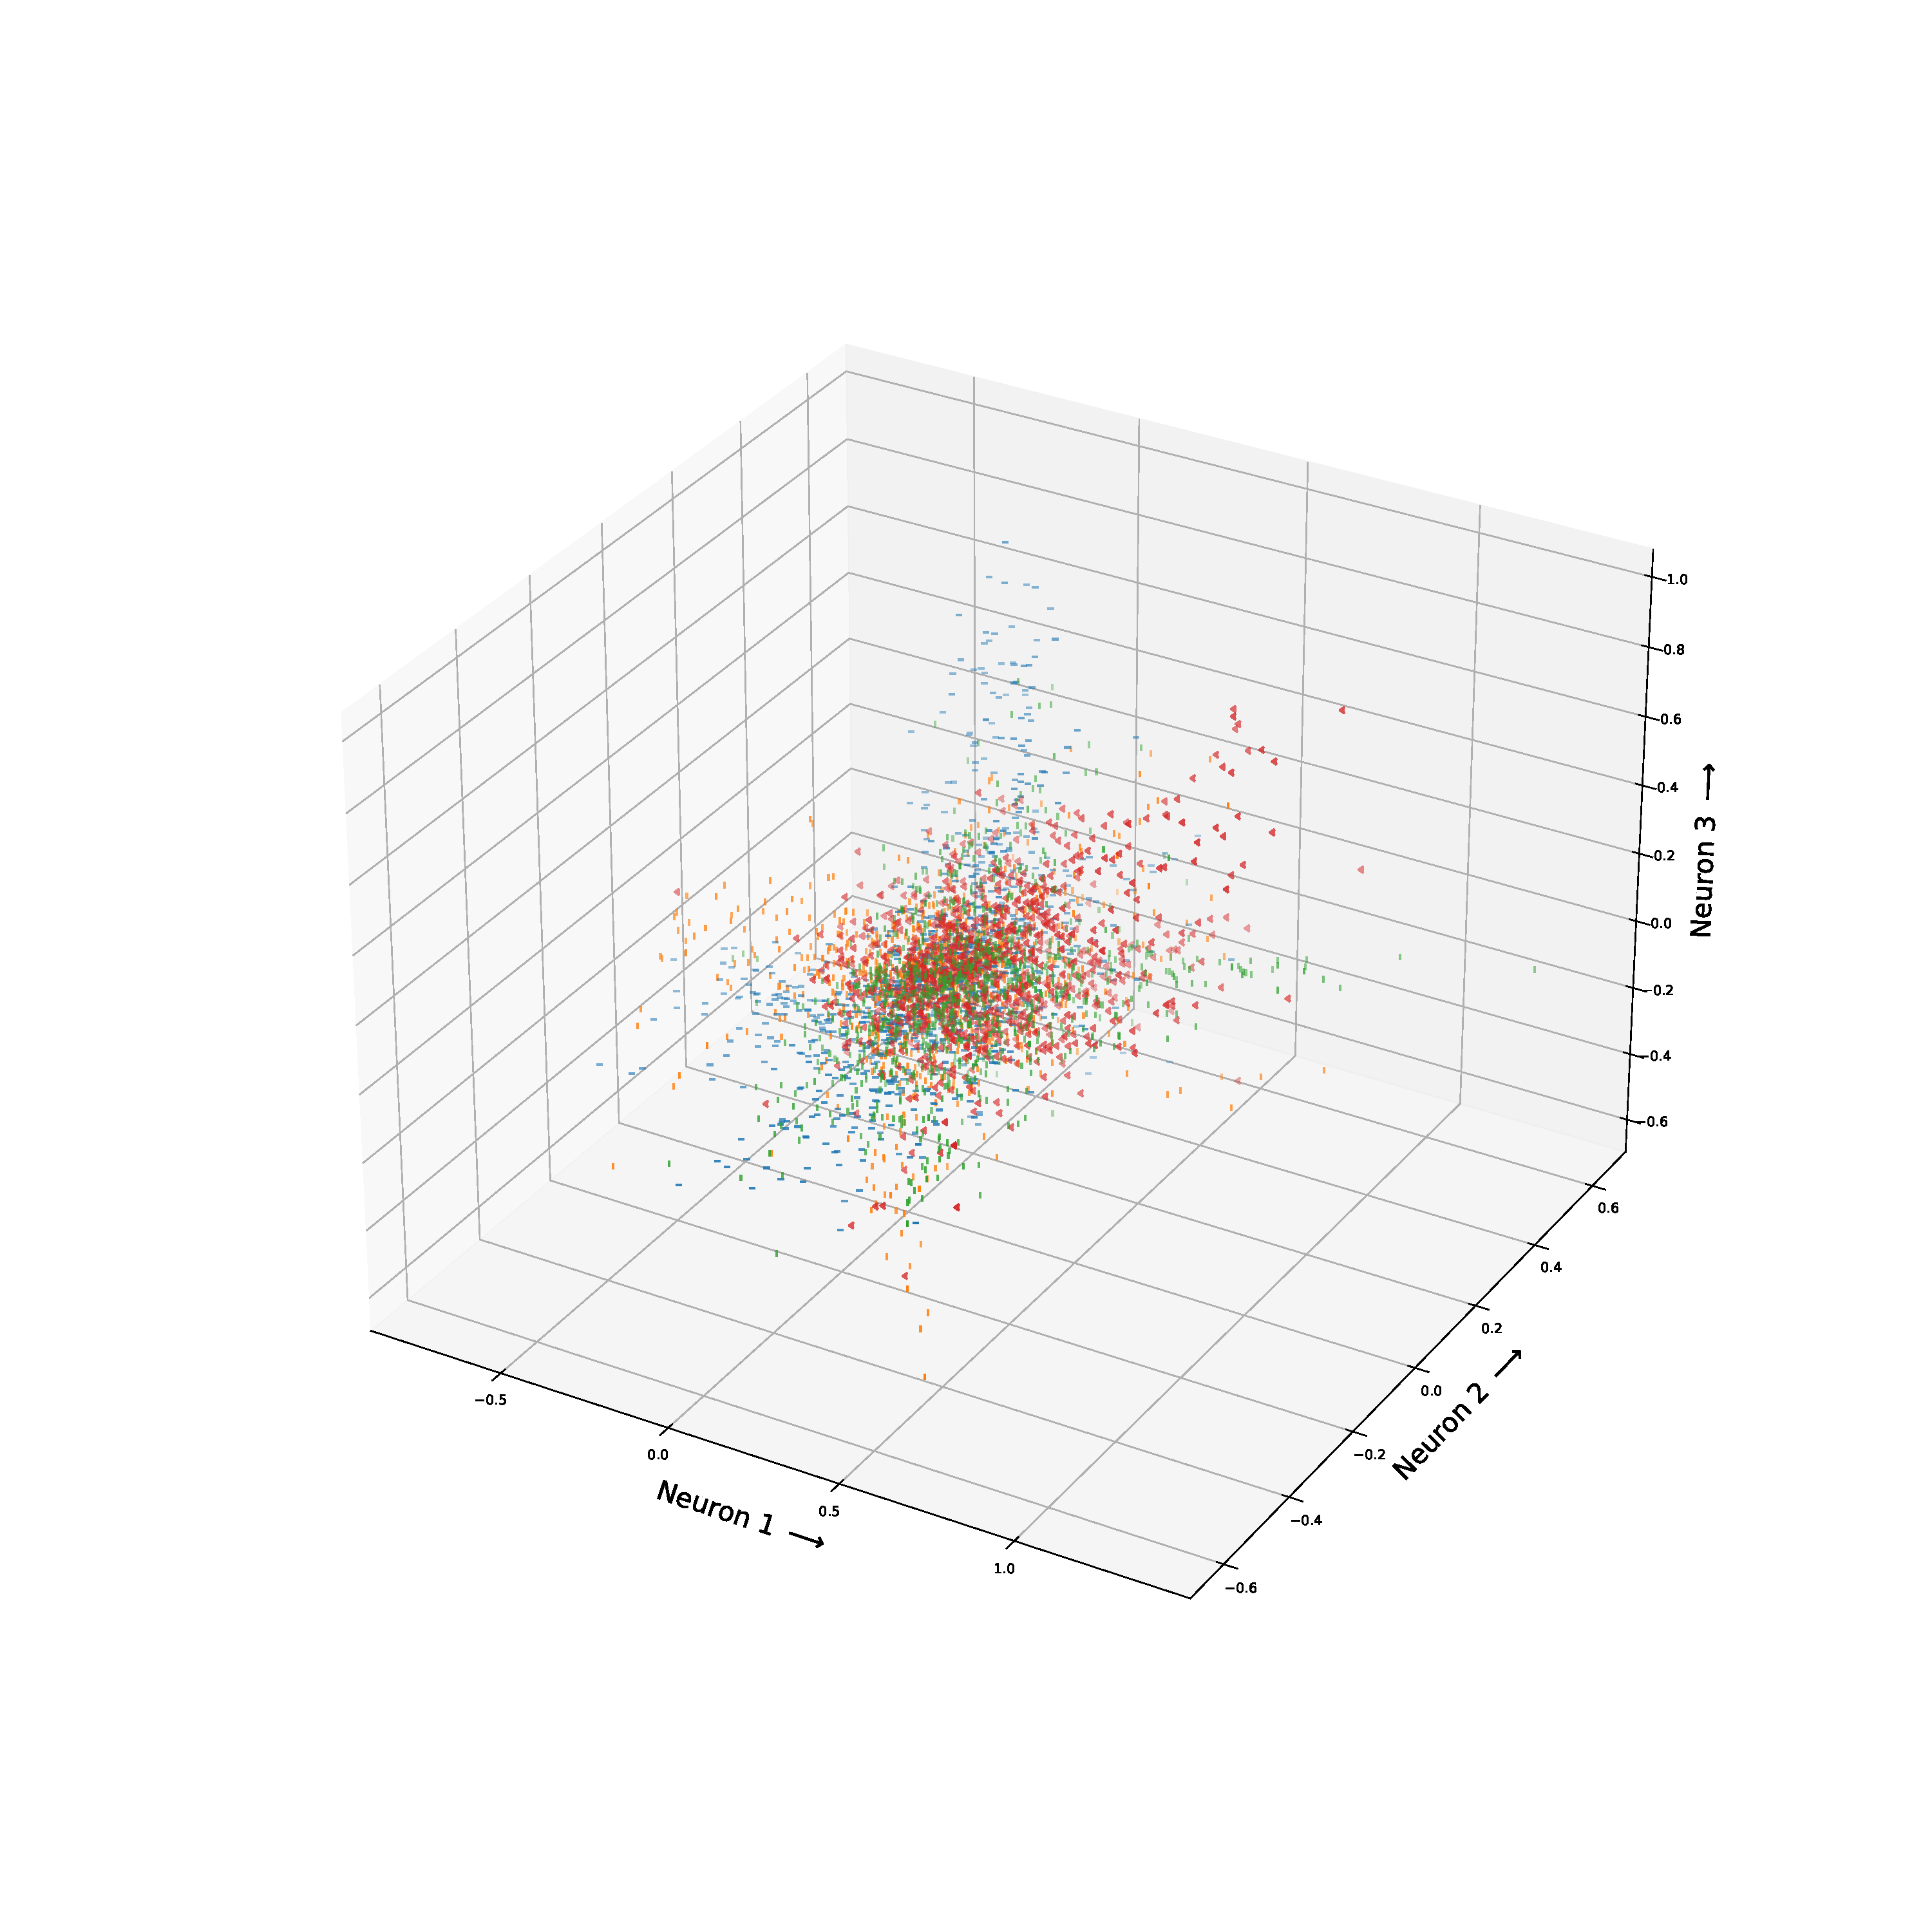
\includegraphics[width=.44\textwidth]{labeled_vs_unlabeled_point_cloud/mmd_epoch0.pdf}
  \hspace{.1cm}
  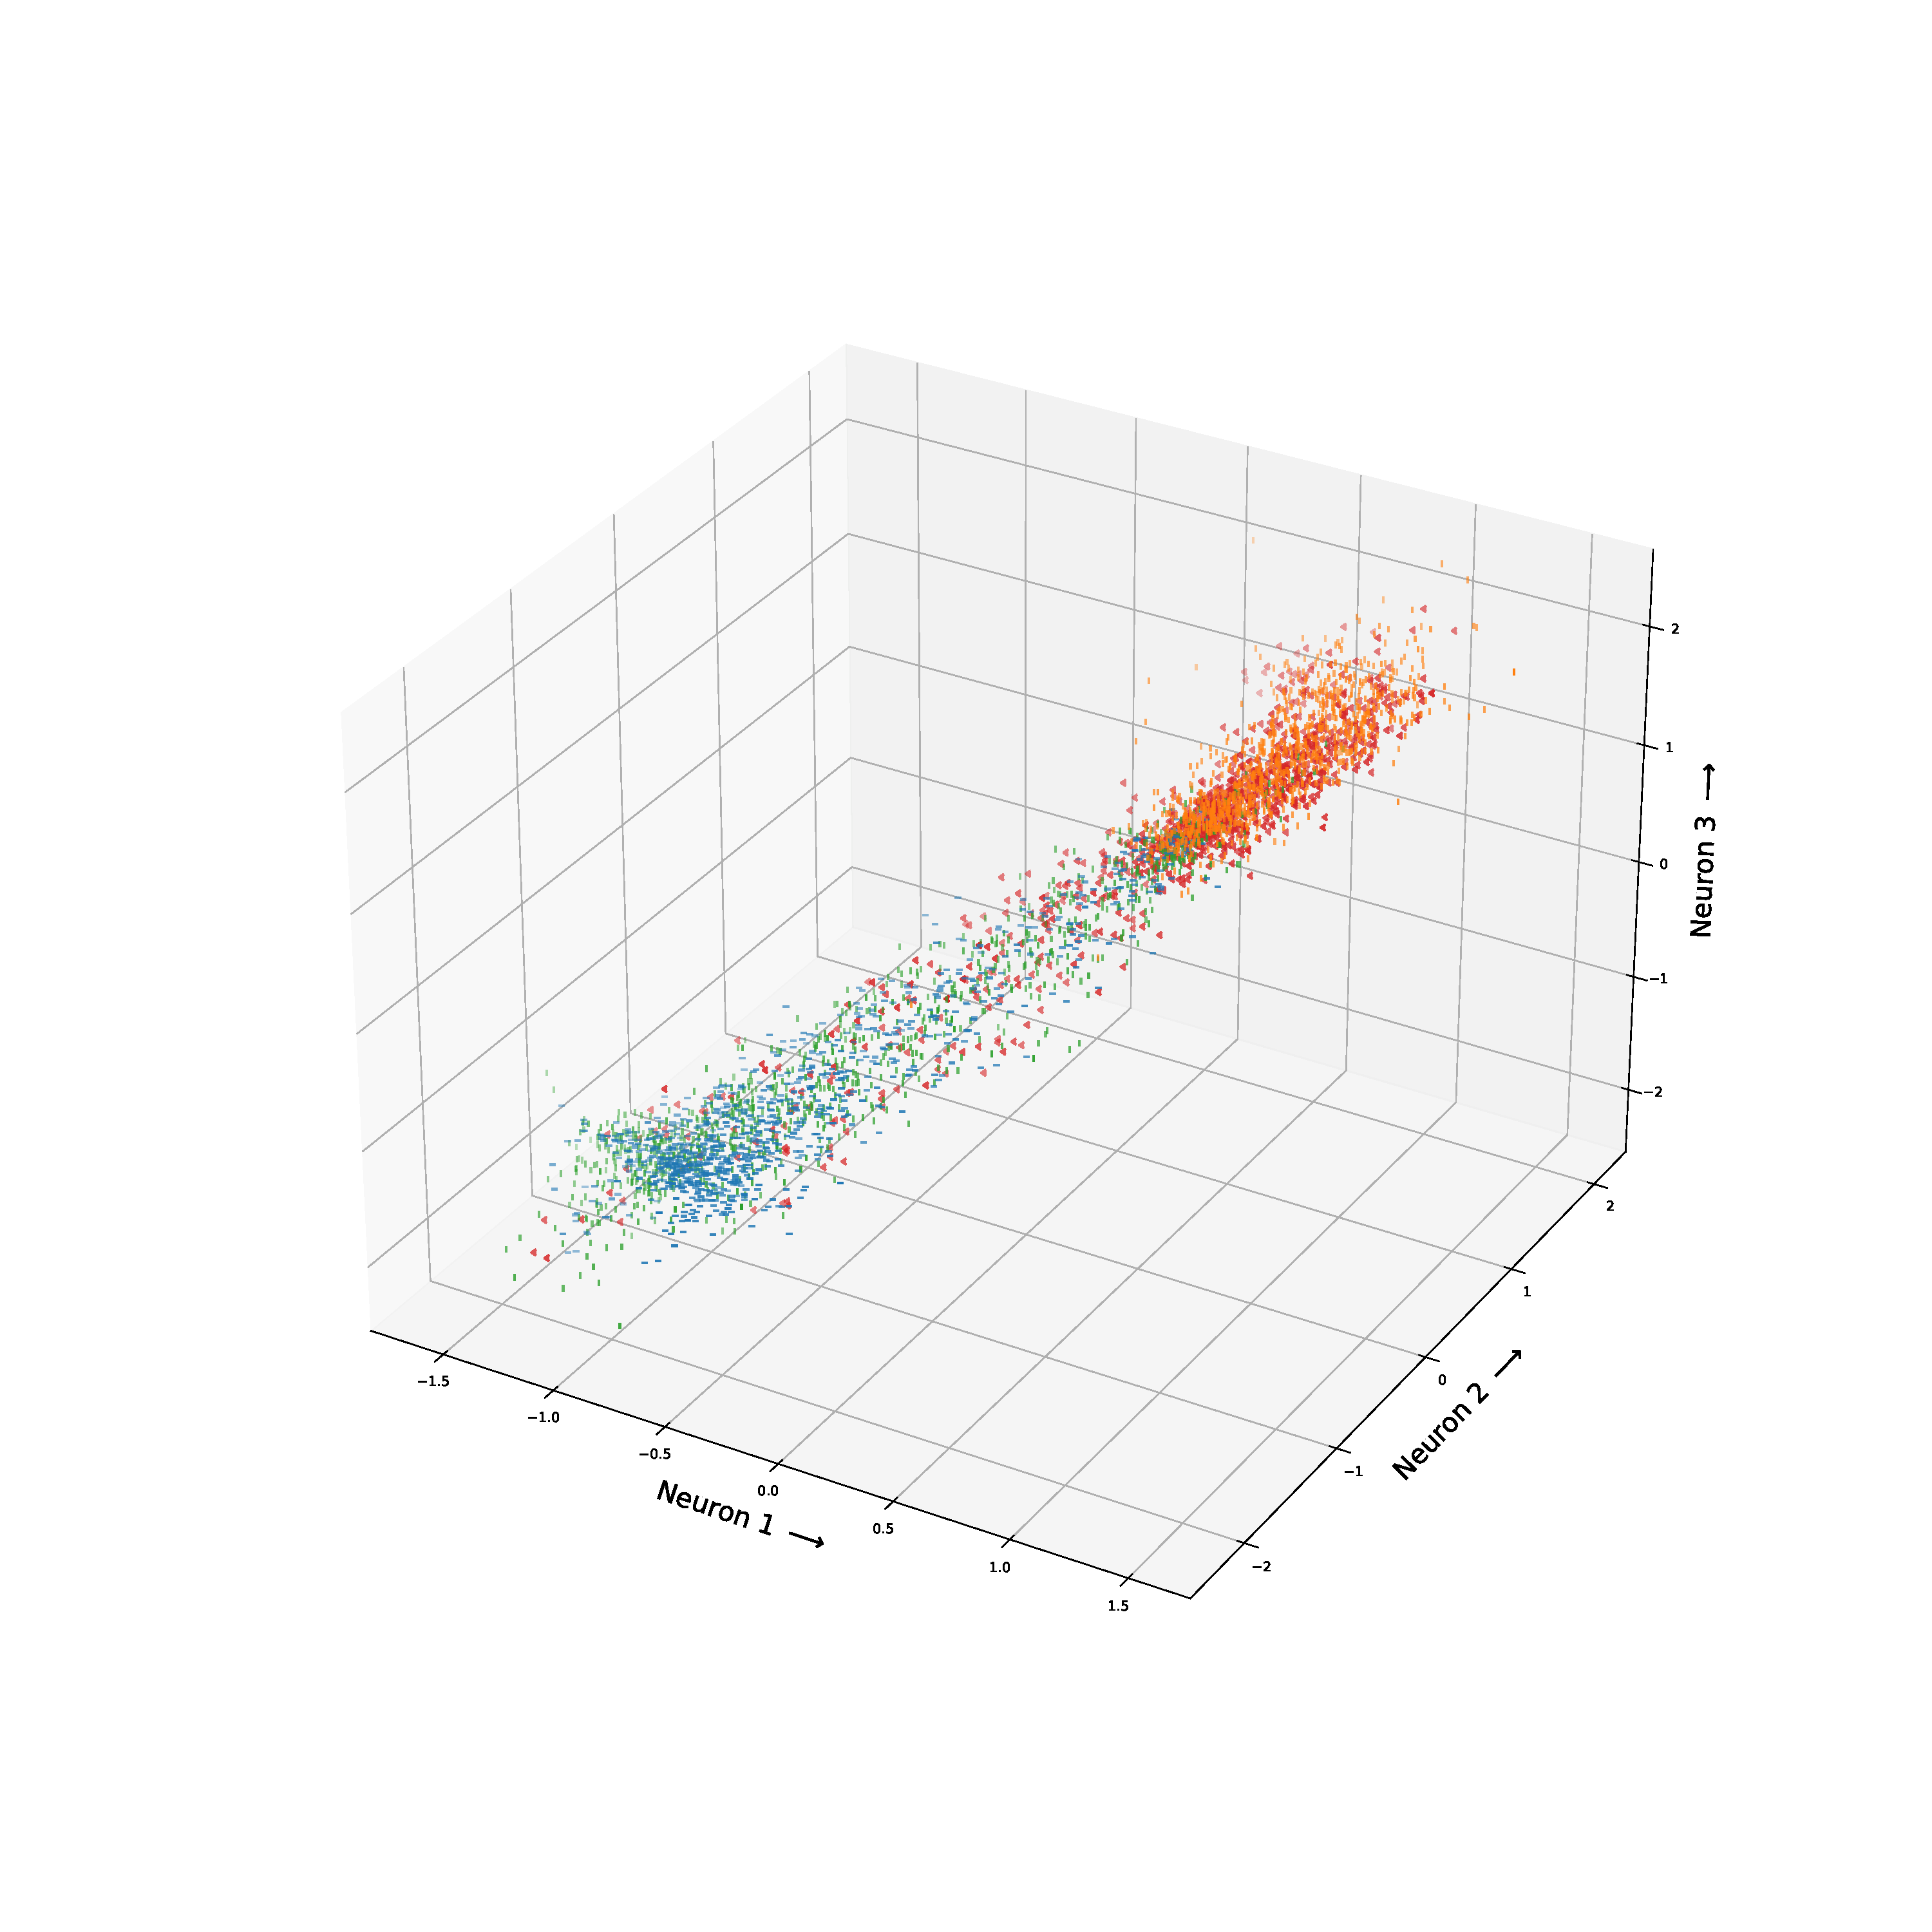
\includegraphics[width=.44\textwidth]{labeled_vs_unlabeled_point_cloud/mmd_epoch6.pdf}

  \vspace{.1cm}
  
  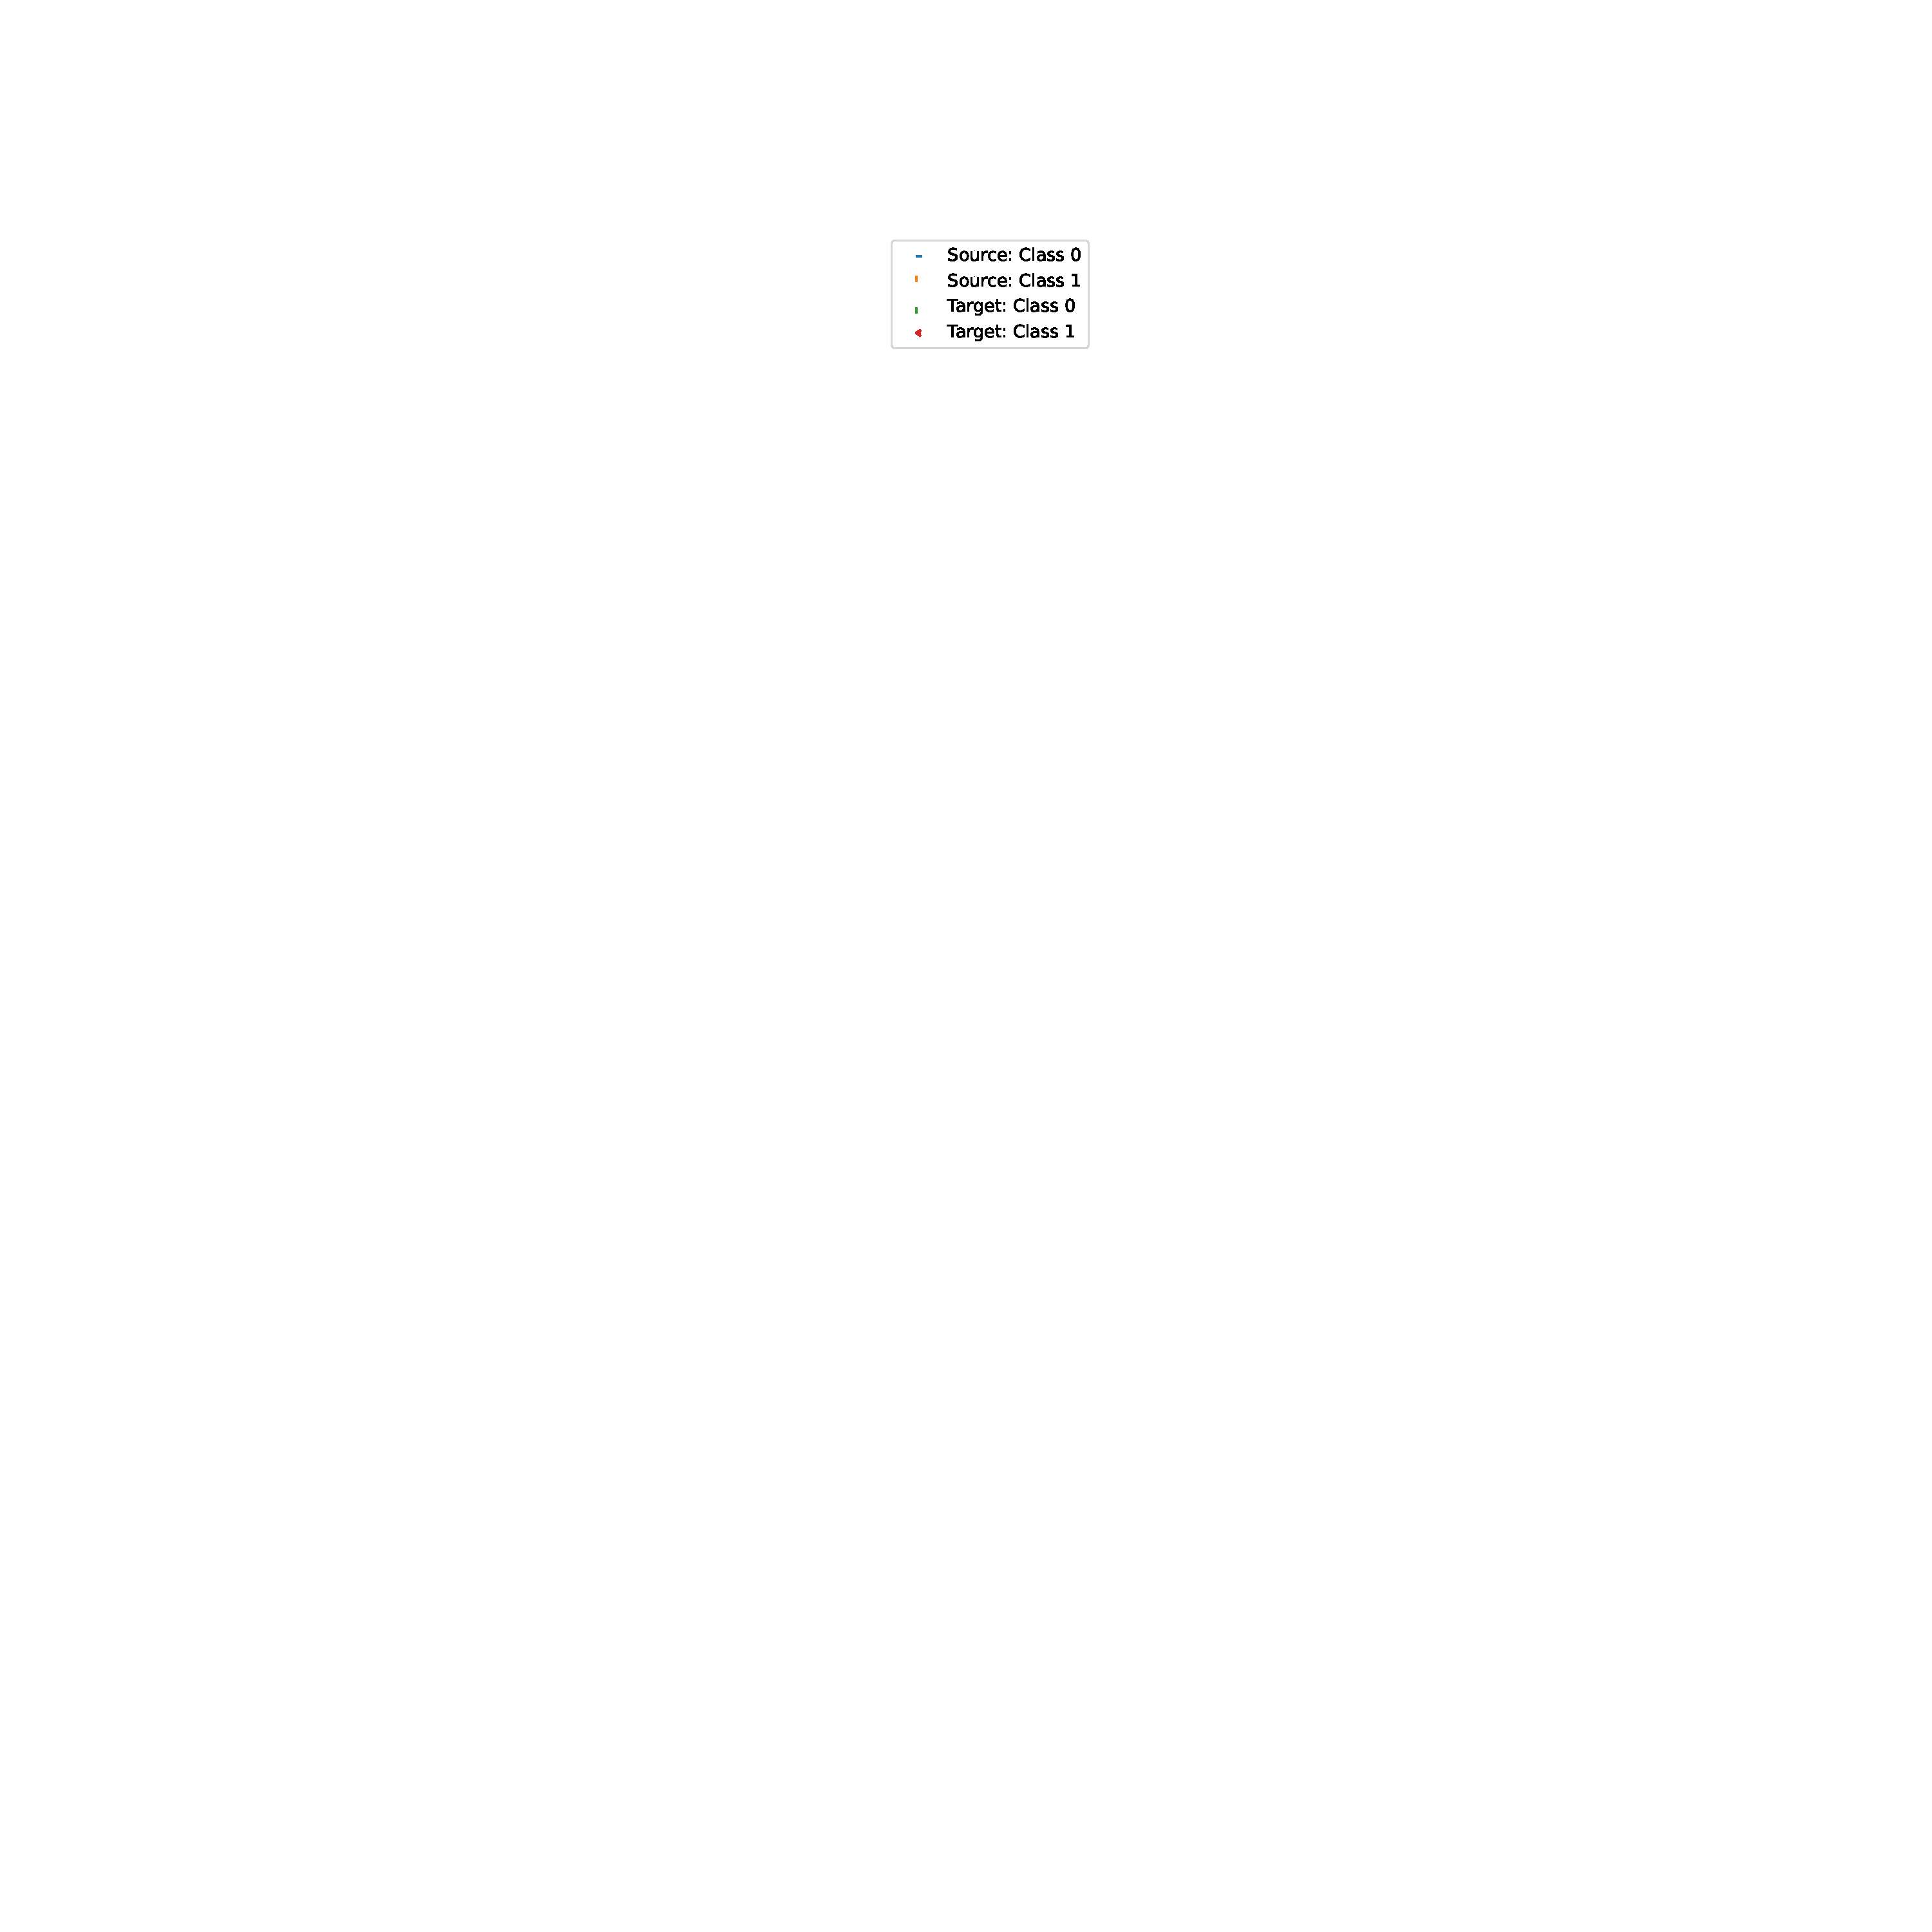
\includegraphics[width=.15\textwidth]{labeled_vs_unlabeled_point_cloud/legend.pdf}

  \caption{Data distribution: labeled (top) vs. unlabeled MMD (bottom) at epoch 0 (left) and epoch 6 (right)}
  \label{fig:point_cloud_labeled_unlabeled_mmd}
\end{figure}

\subsection{Influence of latent feature space choice in MMD loss}
This section analyses the influence of applying the MMD loss to different latent feature maps in the CNN and classifier. The experiments executed for answering this questions are the first which also apply a training in two phases, a phase which trains the whole network with a combination of MMD and source cross-entropy loss and a phase which just optimizes the last two fully connected layers with source cross-entropy loss, as described in section \ref{sec:Proposed_training}. The "regular FC MMD" loss calculates the source and target discrepancy from the three latent feature maps in the classifier (flattened output of CNN, FC1, FC2). The "regular FC + CNN MMD" loss additionally considers the feature maps of the three convolutional layers in the CNN (Conv 1, Conv 2 and Conv 3). The development of the accuracy, the source cross-entropy and MMD loss during the training process are shown in fig. \ref{fig:accuracy_cnn_and_no_cnn_mmd} and fig. \ref{fig:loss_cnn_and_no_cnn_mmd}. The accuracies in source and target domain are higher when including the CNN feature maps into the MMD loss. Besides that, including the CNN feature maps in the MMD loss increases the stability of the training. The losses as well as the accuracies converge faster and smoother.

\begin{figure}[H]
  \centering
  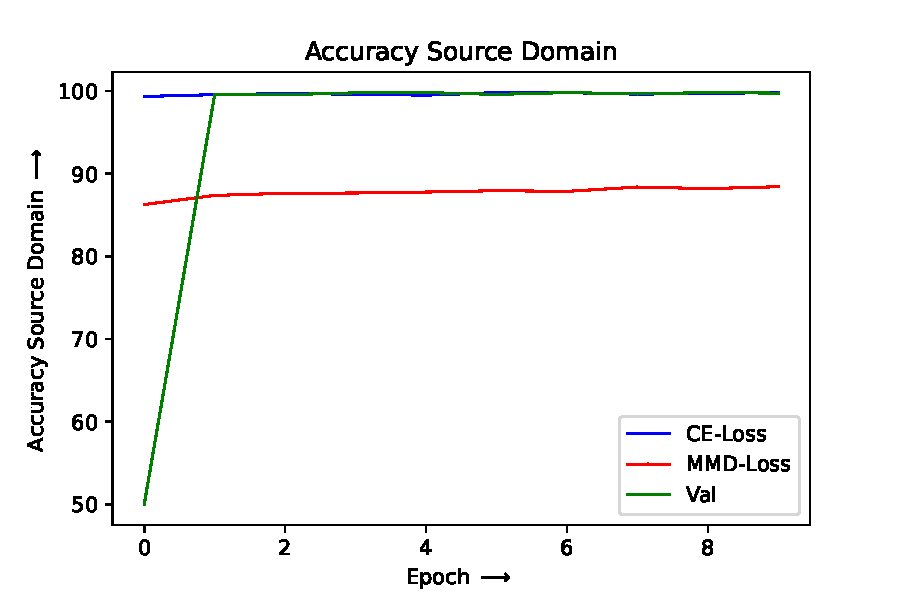
\includegraphics[width=.47\textwidth]{plots_CNN_MMD/Accuracy_Source_Domain_CNN_MMD.pdf}
  \hspace{.3cm}
  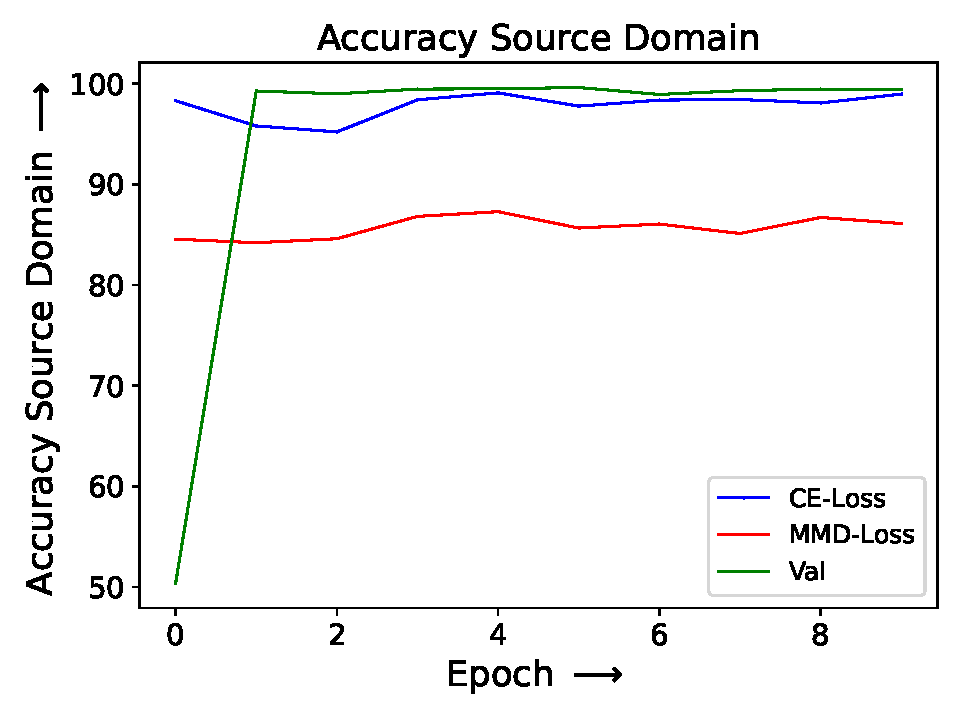
\includegraphics[width=.47\textwidth]{plots_CNN_MMD/Accuracy_Source_Domain_FC_MMD.pdf}

  \vspace{.1cm}

  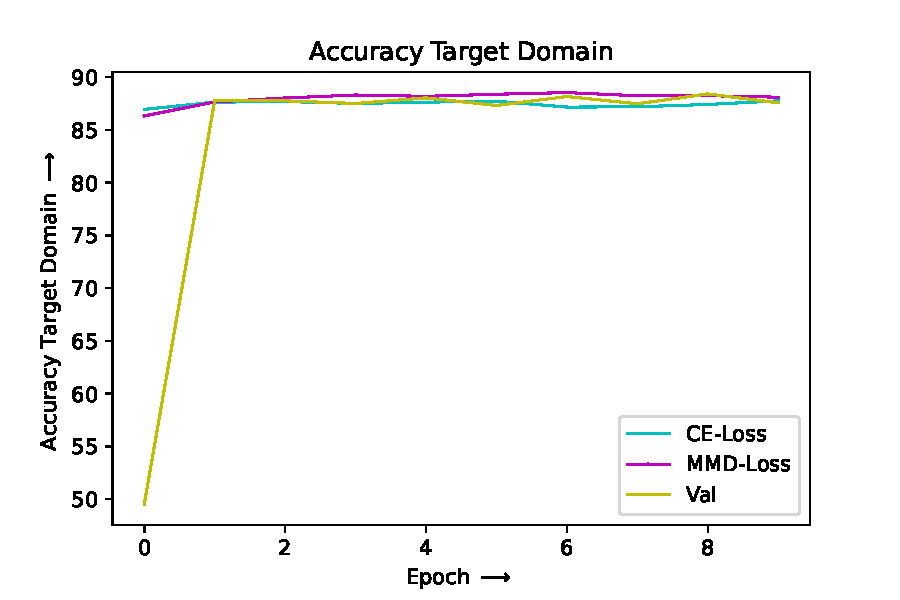
\includegraphics[width=.47\textwidth]{plots_CNN_MMD/Accuracy_Target_Domain_CNN_MMD.pdf}
  \hspace{.1cm}
  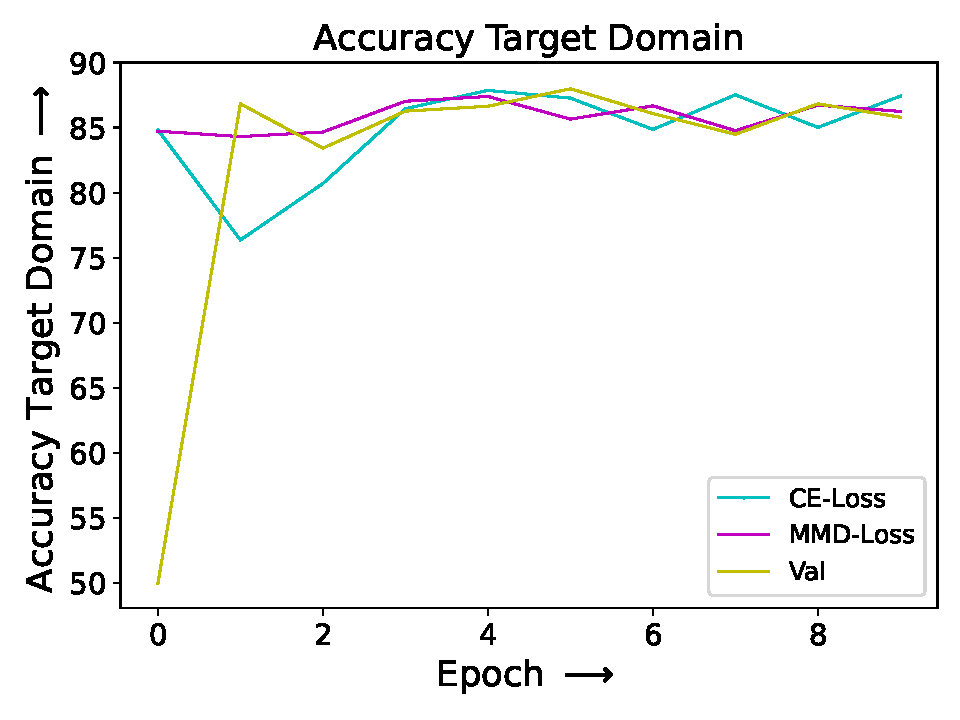
\includegraphics[width=.47\textwidth]{plots_CNN_MMD/Accuracy_Target_Domain_FC_MMD.pdf}

  \caption{Accuracy curves of regular CNN MMD Loss (left) and regular FC MMD Loss (right)}
  \label{fig:accuracy_cnn_and_no_cnn_mmd}
\end{figure}

\begin{figure}[H]
  \centering
  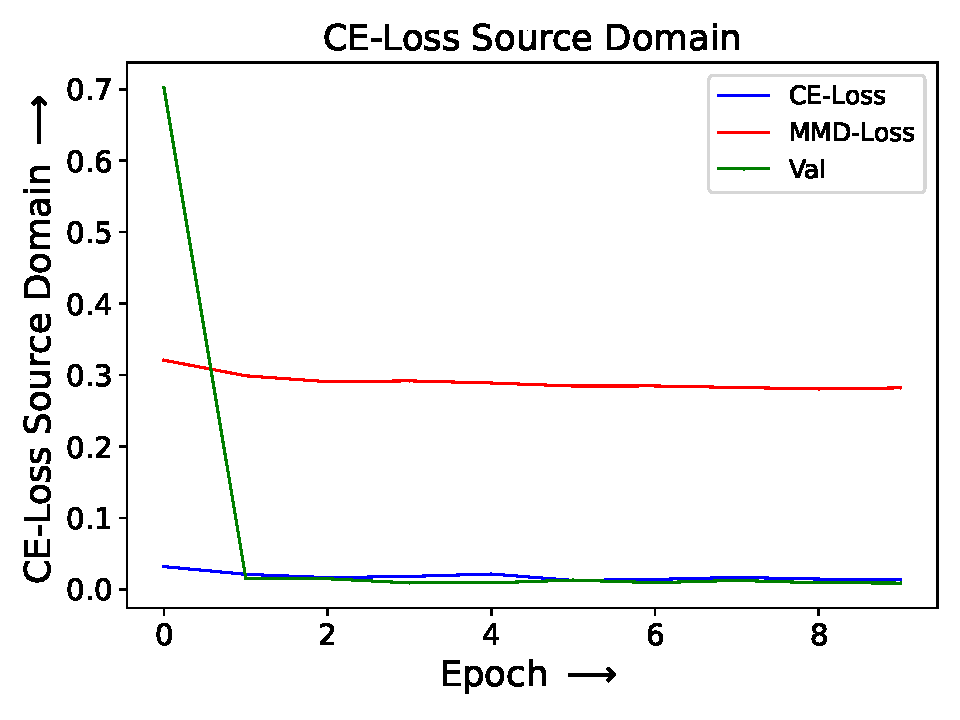
\includegraphics[width=.47\textwidth]{plots_CNN_MMD/CE_Loss_Source_Domain_CNN_MMD.pdf}
  \hspace{.3cm}
  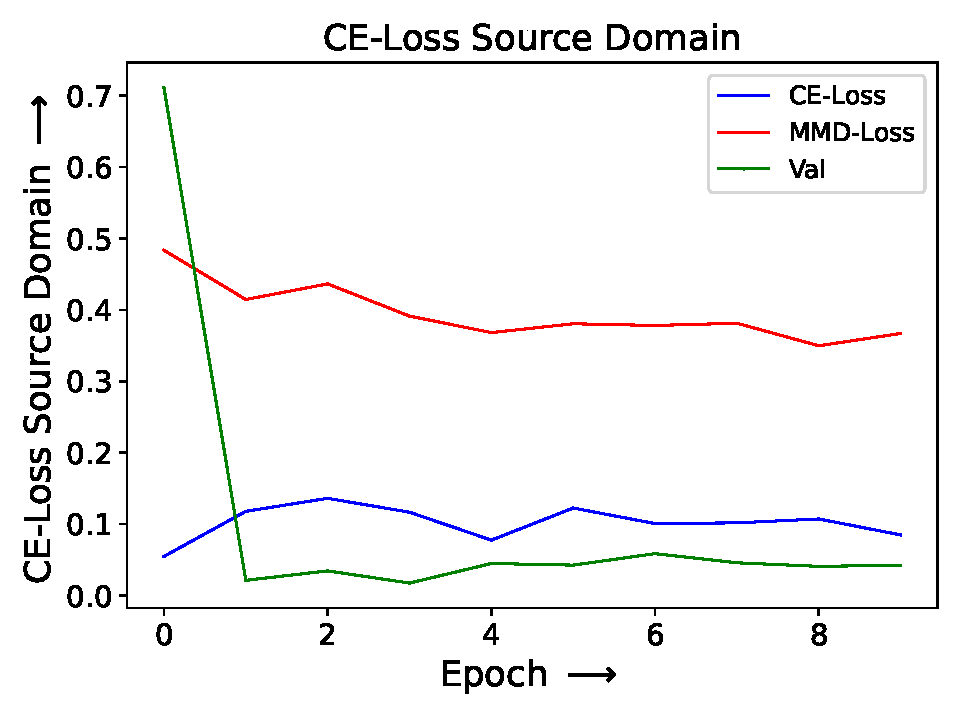
\includegraphics[width=.47\textwidth]{plots_CNN_MMD/CE_Loss_Source_Domain_FC_MMD.pdf}

  \vspace{.1cm}

  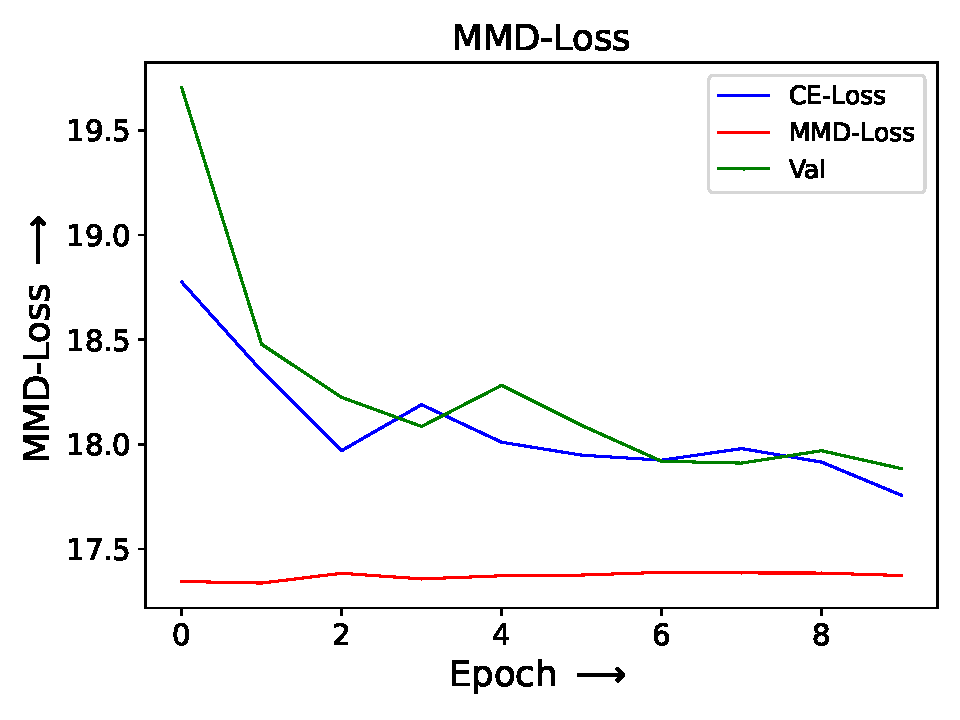
\includegraphics[width=.47\textwidth]{plots_CNN_MMD/MMD_Loss_CNN_MMD.pdf}
  \hspace{.1cm}
  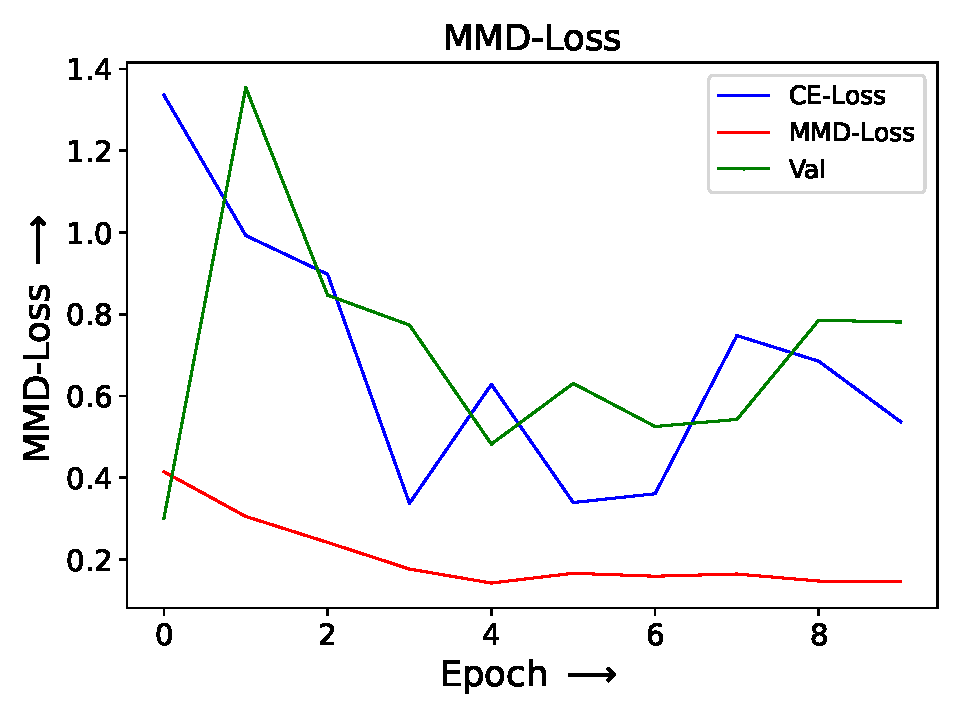
\includegraphics[width=.47\textwidth]{plots_CNN_MMD/MMD_Loss_FC_MMD.pdf}

  \caption{Loss curves of regular CNN MMD loss (left) and regular FC MMD loss(right)}
  \label{fig:loss_cnn_and_no_cnn_mmd}
\end{figure}

By passing data through the model, features with varying levels of abstraction are extracted. The results show that it is reasonable to supervise the domain discrepancy in feature maps of different abstraction levels. Generally shallow layers in neural network extract more global and deeper more task specific features. Deeper layers often suffer more from domain-dependencies. Since each layer in a neural network influences subsequent layers, it makes sense to apply the MMD loss early in the network. Reducing the domain discrepancy in shallow layers makes the network extract more domain-invariant features in these but also all following layers. Especially in challenging tasks with string domain discrepancies it is reasonable to intervene in early layers. Reducing the domain discrepancy in final layers of the model leads to an less stable and smooth optimizations. Potentially, a reason for that could be that the MMD and source cross-entropy loss tend to be more contradicting. The two training goals, which seem to work against each other, make the optimization more fluctuating. During the optimization different strong local minima coming from one of the two losses might be found. The models performance sometimes breaks down after some stable epochs of constant performance increases. One has to remember calculating the regular FC + CNN MMD loss is quiet expansive since the feature maps extracted from the convolutional layers are complex and high-dimensional.



\section{Real world data set}
In the following section the performance of different MMD-based domain adaption approaches are evaluated on the real-world ball screw dataset. The model used for this evaluation is presented in fig. \ref{fig:model_real_data}. From the 49 features in the dataset just three (\verb|'C:x_bottom'|, \verb|'C:y_bottom'|, \verb|'C:z_bottom'|) are used. For this reasons three sequences of length 1024 are fed into the CNN.

\begin{figure}[H]
  \centering
  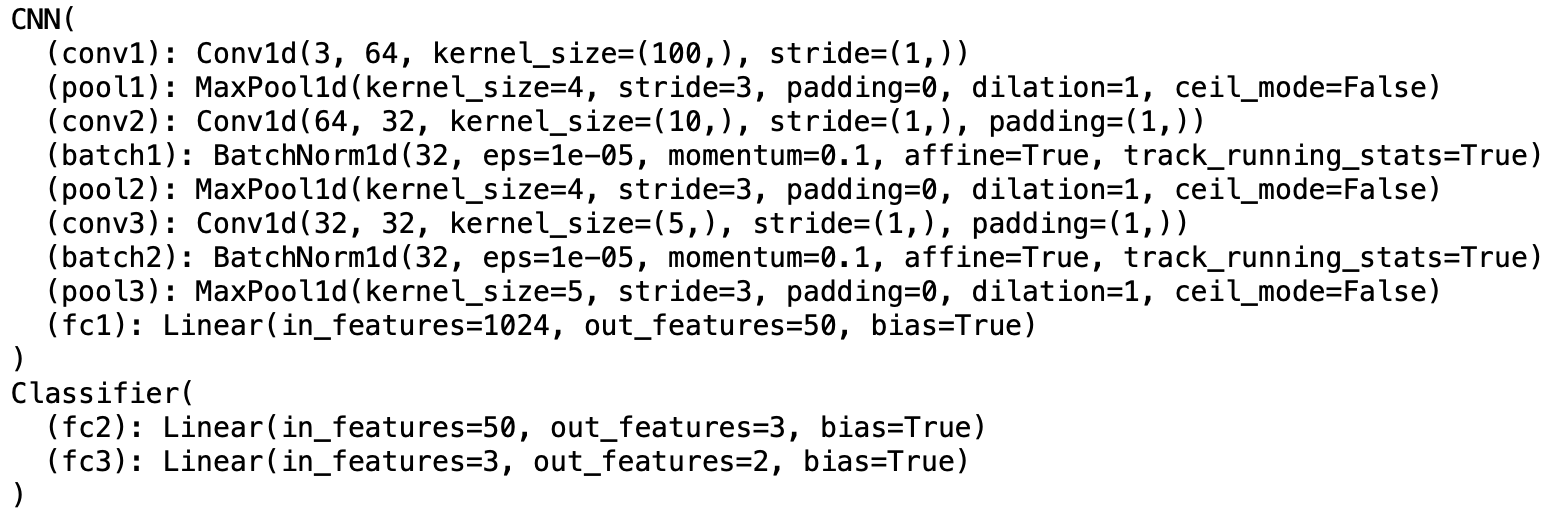
\includegraphics[width=1.1\textwidth]{model_real_data}
  \caption {MMD Model for real data} \label{fig:model_real_data}
\end{figure}


On the real machine dataset the three approaches regular FC + CNN MMD loss,  regular FC MMD and no MMD loss are evaluated. The accuracies on the source and target domain are visualized in fig. \ref{fig:accuracy_real_world}. In each figure three curves are presented representing different phases of the training. During the MMD Loss phase the whole model consisting of CNN and classifier are optimized with a weighted average of MMD and cross entropy loss. In the CE-Loss phase just the classifier is optimized according to a cross-entropy loss. During both phases an ADAM optimizer with a learning rate of 1e-2, beta1 of 0.9 and beta2 of 0.99 is used . In the val phase the model is evaluated. Before the training the data is split for these three phases accordingly (MMD-Loss: 60\%, CE-Loss: 20\%, Val: 20\%). Therefore all experiments follow a proper train validation split. It becomes obvious that the accuracies achieved on the validation set of the target domain were able to be increased with about 10\% by using the two MMD variations. The MMD and cross entropy loss seems to be decreased more smoothly when including CNN features into the MMD loss for the optimization of the model. Also the accuracy achieved on the target validation set achieved the regular FC + CNN MMD loss beat the one achieved with the regular FC MMD loss. Without using any MMD loss the model performance on the target domain could be increased by just around 2\%. When using the regular FC MMD loss sometimes the performance of the model breaks down  little bit. Often times this can be seen in the accuracy of the target and source domain. An example for this phenomena can be seen in fig. \ref{fig:accuracy_real_world} when looking at the accuracies of regular FC MMD (middle). In epoch ~27 the accuracy breaks down on the target and source domain. Especially during the combined training with the MMD and cross entropy loss this effect becomes especially obvious. Like mentioned in previous chapters this shows that when not including the latent features of the CNN in the MMD loss the cross entropy and MMD loss seem to work against each other, which makes the optimization less stable.

\begin{figure}[H]
  \centering
  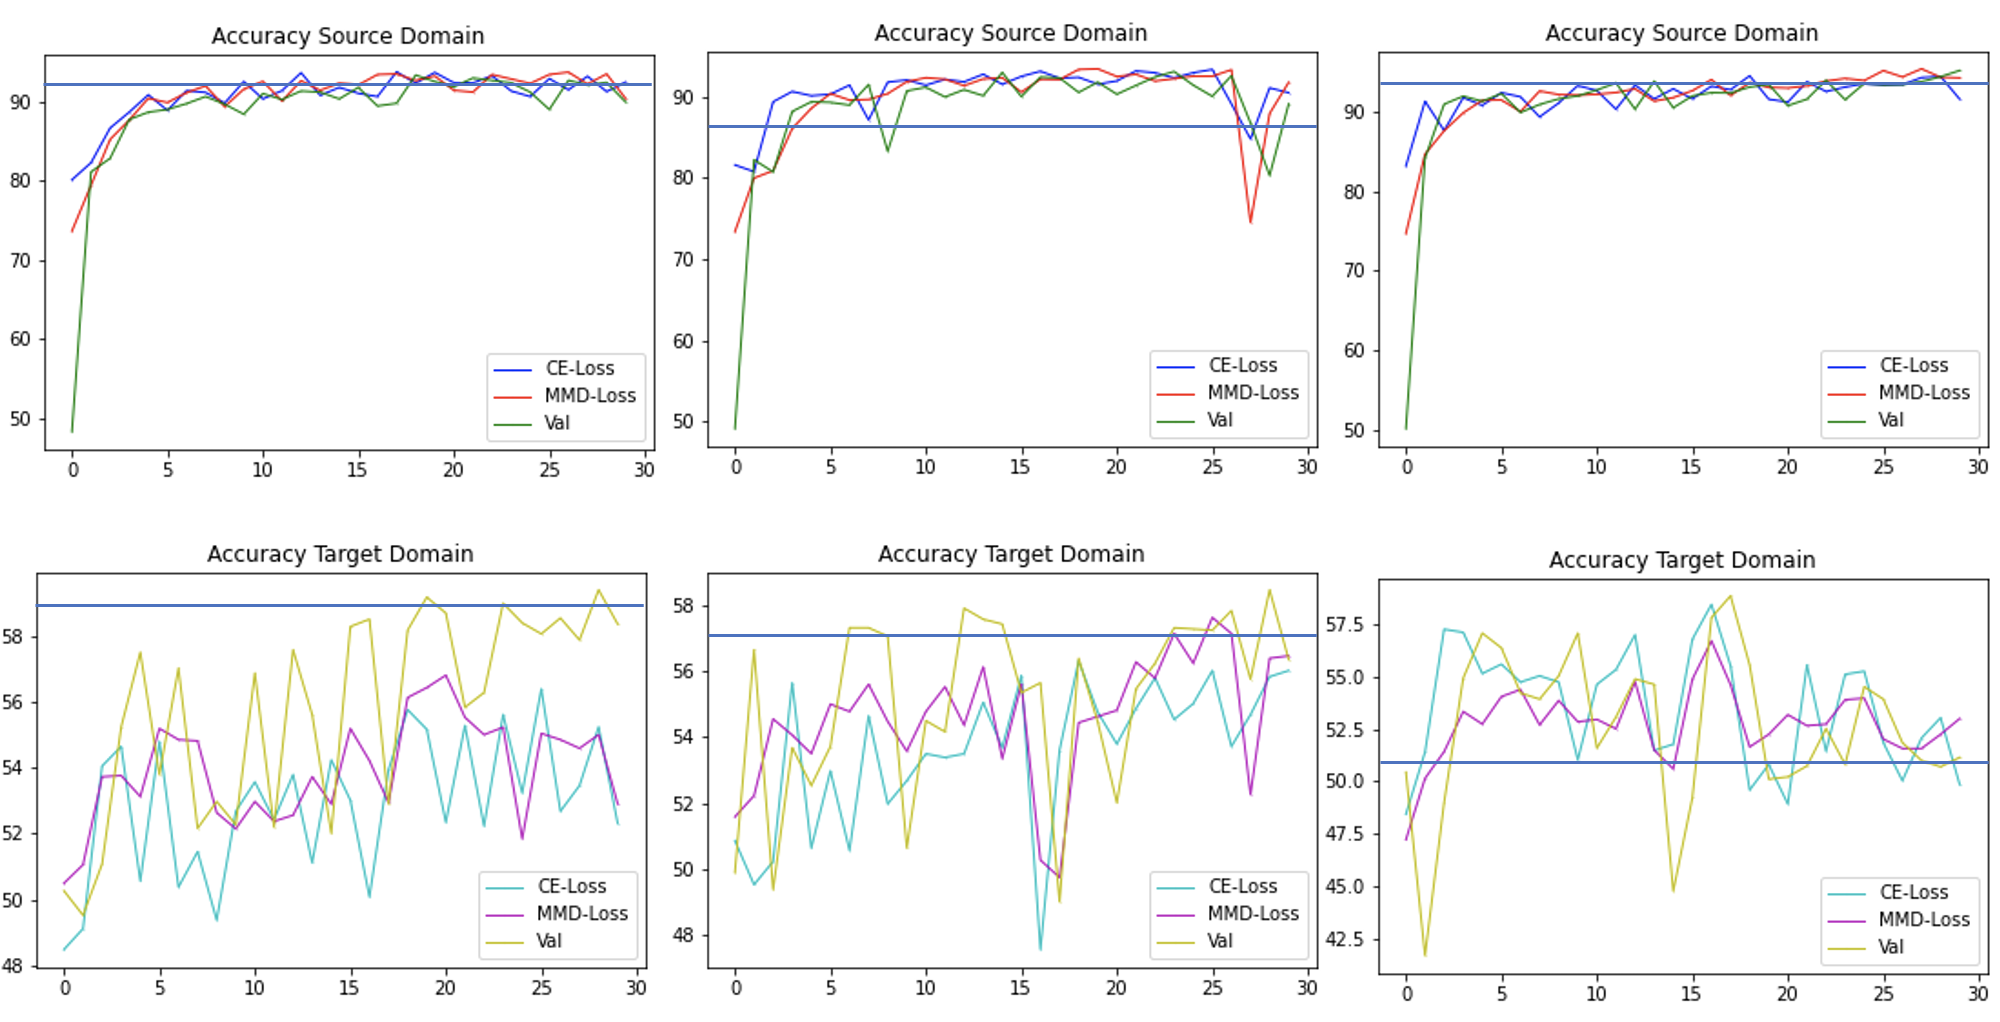
\includegraphics[width=1.1\textwidth]{accuracy_real_world}
  \caption {Accuracies for model training with Regular FC + CNN MMD loss (left), Regular FC MMD (middle) and No MMD loss (right)} \label{fig:accuracy_real_world}
\end{figure}


\begin{figure}[H]
  \centering
  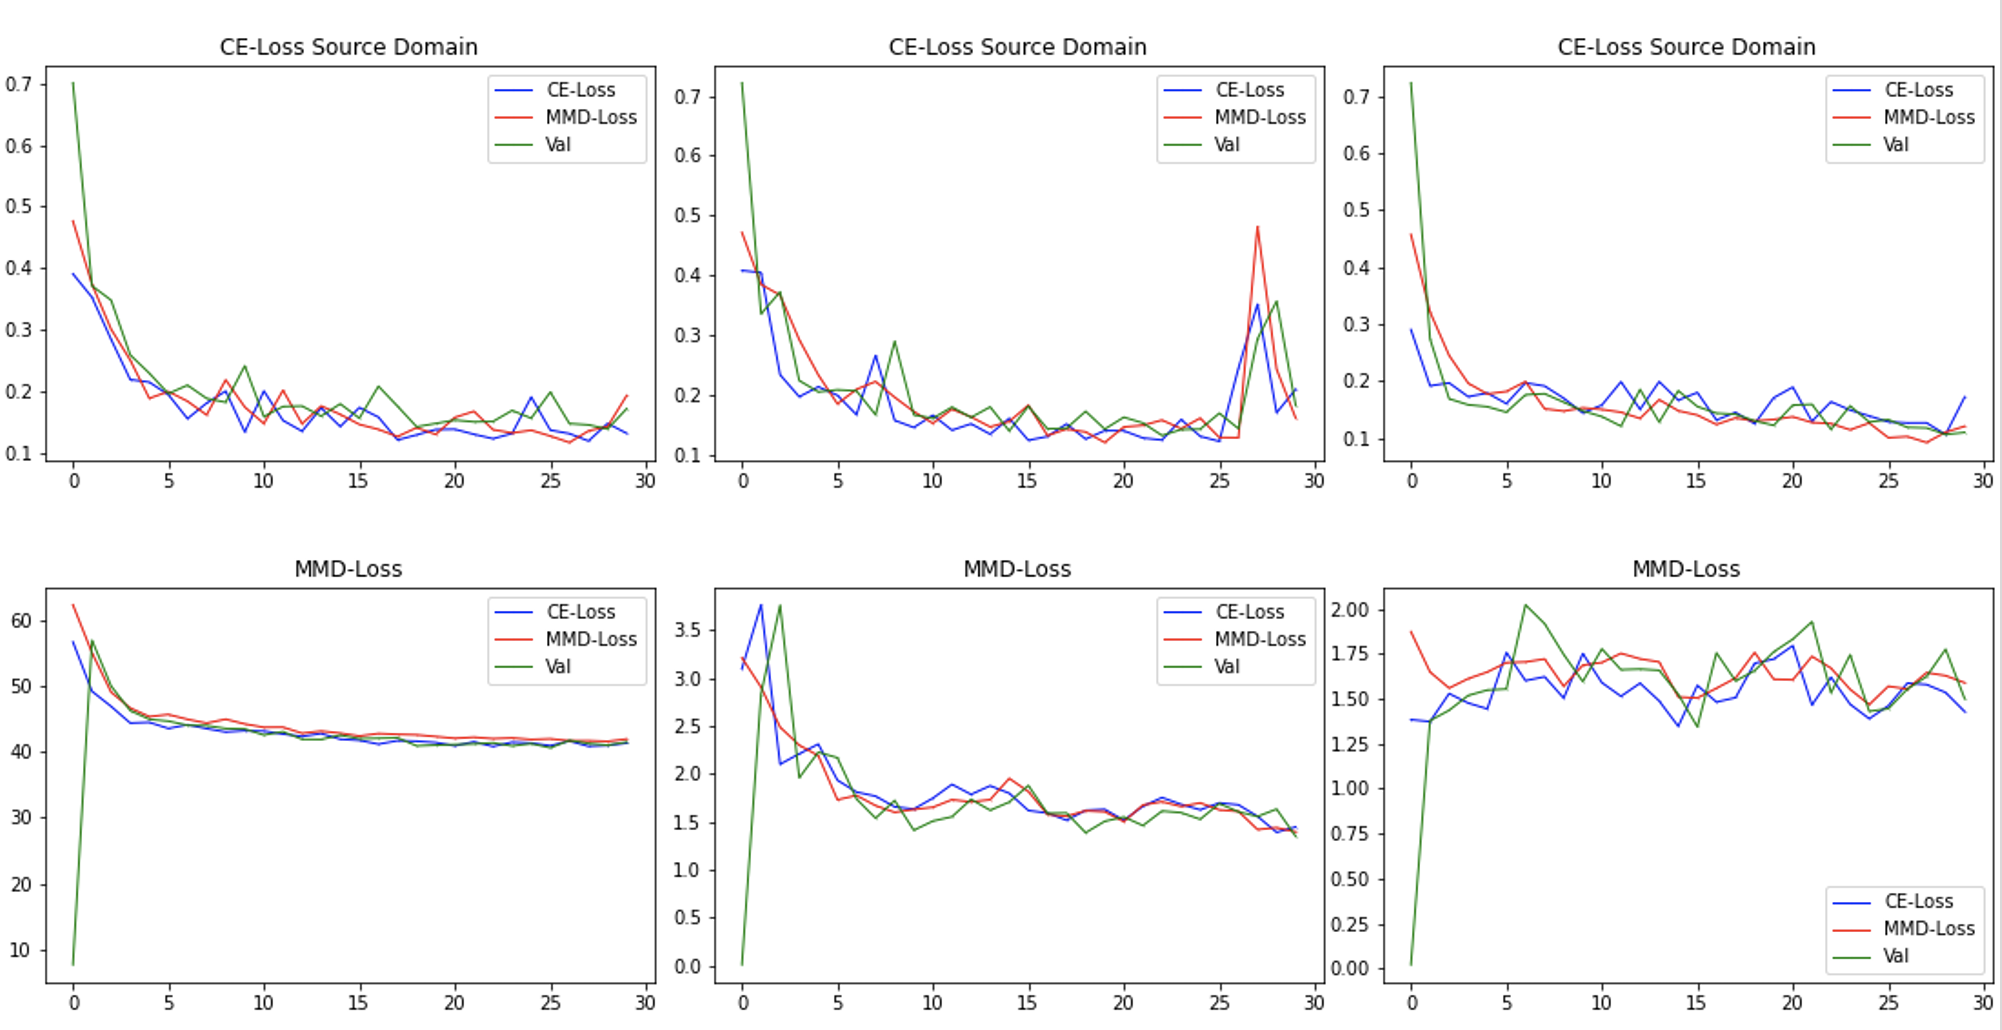
\includegraphics[width=1.1\textwidth]{loss_real_world}
  \caption {Loss for model training with Regular FC + CNN MMD loss (left), Regular FC MMD (middle) and No MMD loss} \label{fig:loss_real_world}
\end{figure}


In fig. the development of the source domain cross entropy MMD loss is shown. It can be seen, that the hyperparameter GAMMA was picked well, such that the MMD as well as the source cross entropy loss were able to be reduced smoothly throughout the trainings process. 


Unfortunately the MMD loss could just minimize the domain discrepancy by a little. The domain discrepancy problem couldn't be solved completely. Still the idea of the MMD loss becomes more clear in the experiments. Also the positive effect of the MMD loss for the training is obvious. For the complex multi-dimensional dataset the MMD loss is probably not sophisticated enough to detect and effectively fight the domain discrepancy.
